\documentclass[14pt,a4paper,titlepage]{extarticle}

\usepackage[utf8]{inputenc}
\usepackage[russian]{babel}
\usepackage[T2A,T1]{fontenc}

\usepackage{titlesec}

\usepackage[left=3cm,right=1.5cm,top=2cm,bottom=2cm]{geometry}
\usepackage{indentfirst}
\usepackage[onehalfspacing]{setspace}
\setlength{\parskip}{6pt}

\usepackage{enumitem}
\setlist[enumerate]{parsep=0pt, parsep=0pt, topsep=0pt, itemindent=\dimexpr\parindent+\labelwidth-\labelsep\relax,leftmargin=0pt}
\setlist[itemize]{label=---, parsep=0pt, topsep=0pt, partopsep=0pt, itemindent=\dimexpr\parindent+\labelwidth-1.5\labelsep\relax,leftmargin=0pt}
\usepackage{amsmath}
\usepackage{amsfonts}
\usepackage{amssymb}
\usepackage[labelfont={small,bf},textfont={small,bf}]{caption}
\DeclareCaptionLabelSeparator{defffis}{ \textbf{--} } % Picture caption separator
\captionsetup{justification=centering,labelsep=defffis}
\addto\captionsrussian{\renewcommand{\figurename}{Рисунок}} % Рис. -> Рисунок
\usepackage{etoolbox}
\makeatletter
\patchcmd{\l@section}
{\hfil}
{\leaders\hbox{\normalfont$\m@th\mkern \@dotsep mu\hbox{.}\mkern \@dotsep mu$}\hfill}
{}{}
\makeatother
\usepackage{graphicx}
\usepackage{subcaption}
\renewcommand{\thesubfigure}{\asbuk{subfigure}}

\usepackage{titlesec}
\usepackage{textcase}
\newcommand{\sectionbreak}{\clearpage}
\renewcommand{\paragraph}[1]{\textbf{#1.}~}
\titleformat*{\section}{\normalsize\bfseries}
\titleformat*{\subsection}{\normalsize\bfseries}
\titleformat*{\subsubsection}{\normalsize}

\setlength{\parindent}{1.25cm}

\usepackage{minted}
\renewcommand{\theFancyVerbLine}{\normalfont \textcolor[rgb]{0,0,0}{\normalsize{\arabic{FancyVerbLine}}}}
\usepackage{courier}
\usemintedstyle{bw}
\newcounter{listingsNumber}
\newcommand{\listingcaption}[1]{\stepcounter{listingsNumber} %
\par \addvspace{0.5\baselineskip
\begin{minipage}{\textwidth-\parindent}
\textbf{Листинг \arabic{listingsNumber} -- #1}%
\end{minipage}
\vspace{-1.3\baselineskip}
}}

\newcommand{\nnumsection}[1]{%
	\clearpage
%	\phantomsection
	\addcontentsline{toc}{section}{#1}
	\section*{#1}
}

\makeatletter
\patchcmd{\FV@SetupFont}
  {\FV@BaseLineStretch}
  {\fontencoding{T1}\FV@BaseLineStretch}
  {}{}
\makeatother

\newcommand\dissername{Разработка метода оптимального частотно-территориального планирования}

\sloppy
\begin{document}
\begin{titlepage}
\centering
МИНИСТЕРСТВО ОБРАЗОВАНИЯ И НАУКИ РОССИЙСКОЙ ФЕДЕРАЦИИ

Государственное образовательное учреждение \\ высшего профессионального образования

\textbf{«Сибирский государственный аэрокосмический университет
имени академика М.Ф. Решетнева» \\ (СибГАУ)}

\vfill

\begin{tabular}{p{0.5\textwidth}l}
ИНСТИТУТ (ФАКУЛЬТЕТ) & \underline{Информатики и телекоммуникаций}\\
НАПРАВЛЕНИЕ & \underline{11.04.02 Инфокоммуникационные }\\
~ & \underline{технологии и системы связи}\\
МАГИСТЕРСКАЯ ПРОГРАММА & \underline{Телекоммуникационные системы и}\\ 
~ & \underline{устройства связи}\\
КАФЕДРА & \underline{Электронной техники и }\\
~ & \underline{телекоммуникаций}\\
\end{tabular}

\vfill

\textbf{МАГИСТЕРСКАЯ ДИССЕРТАЦИЯ}  \\
\textbf{\dissername}

\vfill

\begin{tabular}{p{0.75\textwidth}p{0.25\textwidth}}
{\Large\strut}Магистрант & (Кретинин В.В.)\\
{\Large\strut}Научный руководитель & (Гаипов К.Э.)\\
{\Large\strut}Рецензент &  (Хачатрян Г.Х.)\\
{\Large\strut}Ответственный за нормоконтроль &  (Сухарев Е. Н.)\\
~ & ~ \\
\textbf{Допускается к защите} & ~ \\
{\Large\strut}Зав. кафедрой & (Петров М.Н.) \\
{\Large\strut}«\underline{~~~~~~}»\underline{~~~~~~~~~~~~~~~~~~~~~~~~}2016 г.
\end{tabular}

\vfill
Красноярск 2016 г.
\end{titlepage}
\begin{center}
\textbf{Аннотация работы} \\
В.В. Кретинин \\
~\\
\textbf{\dissername}
\end{center}
Направление 11.04.02 Инфокоммуникационные технологии и системы связи \\
Магистерская программа Телекоммуникационные системы и устройства связи \\
Учебная группа МТК-14-01 \\
Год защиты работы 2016 \\
\par
Одной из проблем, существующих в области беспроводных mesh- и ad-hoc-сетей (сетей ячеистой топологии), является проблема эффективного использования радиочастотного ресурса. С целью решения данной задачи предложена математическая модель и проведены расчеты, показывающие, что подход с использованием адаптивной ширины канала, в противовес текущим решениям с фиксированной шириной канала, является оптимальным с точки зрения обеспечения минимально возможных задержек трафика при передаче данных. 

Модель состоит из линейных уравнений, характеризующих взаимозависимости потоков данных и полос частот каждого канала связи. Вычисления проведены при помощи библиотеки инженерных и научных расчетов SciPy для языка программирования Python. Были получены результаты, показывающие, что перераспределение полос частот использованных радиоканалов позволяет значительно улучшить итоговые характеристики сети, но вместе с тем требует межуровневого подхода к построению стека протоколов. 

\tableofcontents
\nnumsection{ВВЕДЕНИЕ}
Mesh-сеть - это сеть маршрутизаторов, объединенных каналами связи, не образующими ярко выраженной и структурированной топологии, т.е. обладающая «случайными» связями и «ячеистой» топологией. Конечные абоненты сети связаны друг с другом через подключение к маршрутизаторам, но не напрямую. Таким образом, внутри сети выделяются две подсистемы~-- общность связанных между собой маршрутизаторов, выполняющих функцию транзита пользовательских данных, и конечных абонентов, к ним подключаемых [1]. Следует различать mesh-сети с родственным подклассом сетей ячеистой топологии~-- ad-hoc-сетями, в которых подобное разделение отсутствует, а абоненты сети представляют собой одновременно как конечные узлы, так и транзитные. Тем не менее, в контексте маршрутизации они обладают сходными свойствами.

\begin{figure}[h]
	\centering
	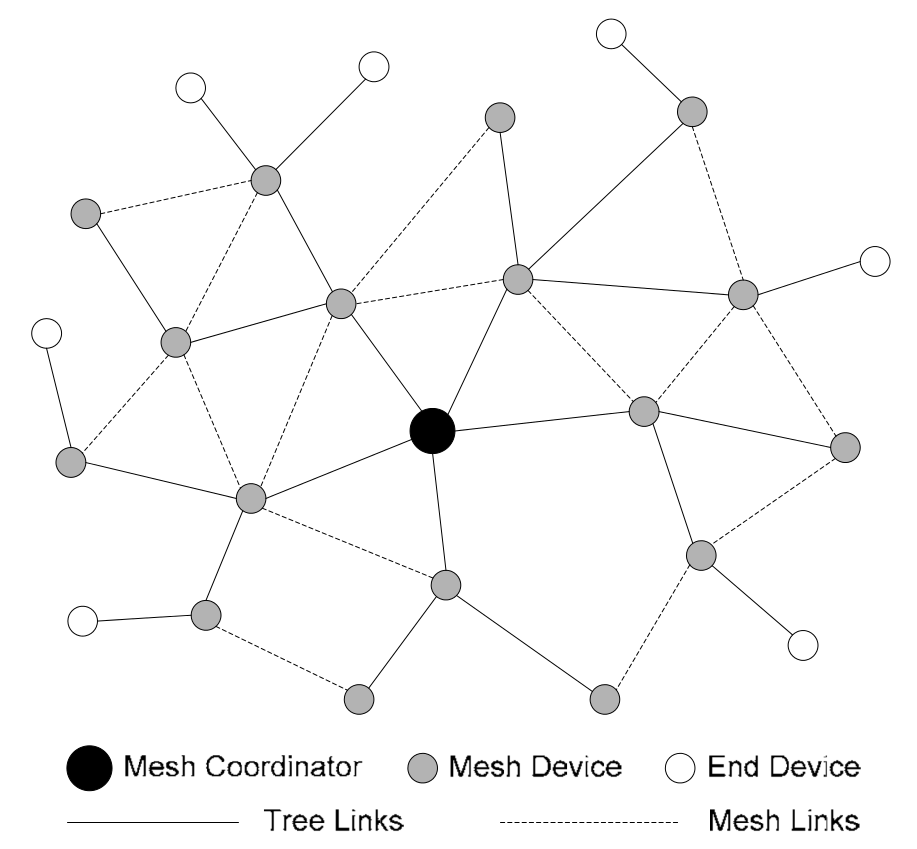
\includegraphics[width=0.6\textwidth]{802_15_5_mesh_topology}
	\caption{Иллюстрация к определению mesh-топологии в стандарте IEEE~802.15.5}
	\label{fig:mesh_topology}
\end{figure}

В настоящее время беспроводные сети ячеистой топологии заняли свое место как в части теоретических исследований, так и промышленно используемых решений. Например, построение mesh-сетей описано в стандартах IEEE 802.11s и IEEE 802.15, а VANET (Vehicular ad-hoc-network, транспортная ad-hoc-сеть)~-- в IEEE 1609 WAVE. Оборудование с поддержкой данного типа сетей выпускается компаниями Cisco (Cisco Meraki) [3], MikroTik [4] и др., среди прочего поддержка mesh-сети присутствует в широкораспространенной ОС для встраиваемых устройств OpenWrt [5].

Основное применение данного типа сетей~-- геология, нефтегазовая промышленность, общественная безопасность и работа в условиях вооруженных конфликтов. Именно в непростых обстоятельствах сети данного типа ведут себя наилучшим образом; их архитектура позволяет учитывать мобильность узлов, сложные конфигурации окружения (замкнутые пространства, плотная городская застройка), а в ряде случаев даже прямое противодействие (постановка помех в процессе ведения боевых действий).

Одной из проблем, существующих в рамках mesh- и ad-hoc-сетей, является проблема эффективного использования ограниченного радиочастотного ресурса. Существующие решения предполагают, что для передачи данных между узлами сети могут варьироваться тип манипуляции, избыточность помехоустойчивого кодирования и алгоритм маршрутизации; при этом ширина канала, используемого для передачи данных между узлами сети с частотным разделением, фиксируется вне зависимости от загрузки и требуемой пропускной способности, что приводит к неэффективному использованию выделенного частотного диапазона. В рамках решения данной проблемы рассмотрены особенности построения mesh-сетей на различных уровнях, предложена математическая модель и проведены расчеты, показывающие, что подход с использованием адаптивной ширины канала, с точки зрения задержек трафика, формирующихся в сети, и загрузки сети является наиболее оптимальным.

\section{ПОДРОБНЕЕ О MESH-СЕТЯХ}
\subsection{История}
Первые беспроводные сети ячеистой топологии строились в 1970 годах как эксперимент, проведенный по заказу Министерства обороны США~-- <<Радиосеть пакетной коммутации>> (Packet Radio Network, PRNET). Затем наработки по данной тематике были использованы в 1980-х гг. в программе создания <<живучей радиосети>> (Survivable Radio Network, SURAN), курируемой агентством по перспективным оборонным научно-исследовательским разработкам США (Defense Advanced Research Projects Agency, DARPA). Целью программ было создание сети пакетной коммутации, отвечающей требованиям высокодинамичной, нестабильной обстановки поля боя.

Для PRNET в качестве протокола доступа к среде использовалось сочетание протоколов ALOHA и CSMA и маршрутизация с применением вектора расстояния (distance-vector routing). Для преемника данного проекта, SURAN, были значительно улучшены массогабаритные и радиочастотные характеристики устройств, масштабируемость алгоритмов и устойчивость к атакам. Протоколы маршрутизации были основаны на подходе, использующем иерархическое состояние канала (link-state routing).

Третья волна интереса возникла в 1990-х гг. Появились доступные ноутбуки, ПО с открытым исходным кодом, появилось долговечное и недорогое радиооборудование инфракрасного и СВЧ диапазонов. Был предложен концепт коммерческого (невоенного) использования сетей ячеистой топологии. 

С другой стороны, в то же время Министерство обороны США спонсировало несколько научно-исследовательских программ: <<Глобальные Мобильные Информационные Системы>> (Global Mobile Information Systems, GloMo), и <<Быстроразвертываемое цифровое радио>> (Near-term Digital Radio, NTDR). Целью GloMo было обеспечение Ethernet-совместимого соединения в офисном окружении для карманных устройств. Доступ к каналу был на этот раз реализован с помощью CSMA/CA и TDMA. NTDR использовало кластеризацию и маршрутизацию по состоянию канала и самоорганизовывалось в двухуровневую сеть.

Вместе с растущим интересом к сетевым технологиям mesh-сетей  к концу 1990-х гг. образовался набор инициативных групп по стандартизации, также было выпущено некоторое количество коммерческих стандартов. Внутри IETF образовалась рабочая группа по мобильным ad-hoc-сетям (Mobile Ad Hoc Networking, MANET), занимающаяся разработкой и внедрением протоколов маршрутизации для сетей ячеистой топологии. Результаты дальнейшего развития плавно переходят в наши дни и описаны во введении.

\subsection{Особенности mesh-сетей}

\paragraph{Многоскачковость}
Mesh-сеть -- децентрализованная сеть, которая обеспечивает прямое соединение между любыми двумя узлами при соответствующих условиях распространения волн и мощности передатчиков. Если прямого соединения между отправителем и получателем не существует, используется маршрутизация с многократной ретрансляцией. В таком случае пакет передается от одного узла другому до тех пор, пока не достигнет назначения. 

Одной из целей, достигаемых с помощью mesh-сетей, является увеличение дальности соединения беспроводной сети без жертвования емкостью канала. Другой важной целью является предоставление соединения абонентам за пределами прямой видимости. Для реализации данных требований многоскачковость является незаменимой возможностью, которая обеспечивает большую пропускную способность без угрозы эффективному использованию радиосреды на коротких дистанциях радиоканалов, меньшую интерференцию между узлами, и более эффективное повторное использование частоты. 

\paragraph{Спонтанная установка связи и способность к самоинициации, коррекции и самоорганизации}
Спонтанная сетевая активность увеличивает производительность сети с помощью гибкой сетевой архитектуры, легкого развертывания и конфигурирования, устойчивости к отказам. Благодаря этим аспектам mesh-сети имеют низкие начальные затраты и хорошую масштабируемость.

Реализация подобной устойчивости и адаптивности является нетривиальной задачей, поэтому среди недостатков данных сетей выделяют прежде всего ресурсозатратность (из-за применения высокоэффективных методов кодирования, частой смены конфигурации сети и необходимости обеспечения быстрой сходимости к  квазиоптимальному решению), что задает требования к производительности устройств и, в случае носимой электроники, энергопотреблению и энергосбережению. Однако вышеозначенные проблемы не являются фундаментальными, а ограничиваются скорее возможностями современной промышленности; кроме того, в течение как минимум последнего десятилетия заметен серьезный рост производительности мобильной электроники, что, при продолжении тренда, может сделать сети ячеистой топологии в будущем гораздо более популярным и обыденным решением, нежели в наши дни.

\paragraph{Мобильность зависит от типа mesh-узлов}
Mesh-маршрутизаторы обычно обладают низкой мобильностью, в то же время клиенты могут быть как стационарными, так и мобильными узлами. Таким образом, мобильность внутри сети отличается для каждого узла.

Из-за возможности быстрого перемещения узлов и изменения условий распространения сетевая информация, в частности, таблица маршрутизации устройств, быстро устаревает. Частое изменение конфигурации сети может вызвать частый обмен контрольной информацией, необходимый для отражения текущего состояния сети, однако из-за малого время жизни такой информации большие пересылаемые объемы служебных пакетов могут никогда на практике не понадобиться. Таким образом, часть пропускной способности, используемая для передачи маршрутизирующей информации, будет потрачена впустую. 

\paragraph{Зависимость энергопотребления от типа mesh-узлов}
Mesh-маршрутизаторы обычно не обладают строгими ограничениями по энергопотреблению, в отличие от клиентов, как правило представляющих собой крайне ограниченные по производительности и энергодолговечности устройства: датчики или карманные приемопередатчики.

\section{СТЕК ПРОТОКОЛОВ}
\subsection{Физический уровень}
Протоколы физического уровня стремительно развиваются в виде теоретических моделей, алгоритмов цифровой обработки сигналов, радиочастотных технологий и проектирования схем для беспроводной связи. Методики в основном сосредоточены на трех направлениях: повышение скорости передачи данных, улучшение устойчивости к ошибкам в беспроводной среде, а также гибкость программного обеспечения радиостанций.

Для повышения пропускной способности беспроводных сетей были изобретены различные высокоскоростные методики физического уровня. Например, мультиплексирование с ортогональным частотным разделением каналов (OFDM) помогло значительно увеличить скорость оборудования IEEE 802.11~-- с 11 до 54 Мбит. Гораздо более высокая скорость передачи данных может быть достигнута с помощью технологии сверхширокополосности (Ultra-Wideband, UWB). Тем не менее, UWB применимо только в случае коротких расстояний, например, в беспроводных персональных сетях (WPAN). Если необходима высокая скорость передачи данных на большем расстоянии, например, в WLAN или WMAN, используются другие физические методы, такие, как механизм с множеством входов и множеством выходов (MIMO). 

Чтобы улучшить устойчивость к ошибкам, было разработано много схем канального кодирования. Так как состояние канала изменяется, схема фиксированного кодирования канала не является эффективной. Таким образом, необходима адаптивная схема кодирования канала. Например, в сотовых сетей 3G и IEEE 802.11a схема кодирования варьируется вместе с изменением состояния канала.

Еще одним направлением является разработка физического уровня таким образом, чтобы радиочастотные характеристики можно было контролировать с помощью программного обеспечения. Такая возможность дает множество преимуществ. Например, методы физического уровня могут быть адаптивно оптимизированы в соответствии с переменными условиями окружающей среды, так что научные исследования и производственный цикл может быть значительно сокращен, приемопередатчик может быть перенастроен и так далее. В общем, данный род технологий объединяется понятием «программно-определяемое радио» (Software-Defined Radio, SDR). В случае использования данной методики ограниченный беспроводной спектр может быть использован гораздо эффективнее.

Методы физического уровня, как правило, касаются только одного канала связи точка-точка. Однако, когда они применяются к беспроводным mesh-сетям, возникают новые комплексные проблемы, которые ухудшают их производительность в среде беспроводной ячеистой сети. Таким образом, научные проблемы, связанные с физическим уровнем, указаны в этой главе. Обсуждаются также пути решения этих проблем.

\subsubsection{Адаптивная модуляция и кодирование}
В канале беспроводной сети существуют два классифицируемых по влиянию вида изменений:
\begin{itemize}
\item Серьезные изменения вызваны зависимостью затухания в тракте передачи от расстояния между передатчиком и приемником и изменчивостью средней величины потерь на трассе;
\item Небольшие изменения вызваны быстрыми колебаниями мощности принимаемого сигнала в течение короткого периода времени или колебаниями пройденного радиоволной расстояния вследствие многолучевого распространения. В широкополосной сети такие быстрые изменения могут привести к частотно-селективным замираниям.
\end{itemize}

Если используются единственный способ кодирования и схема модуляции, то, из-за изменений качества канала связи, скорость появления ошибочных битов в канале значительно изменяется, что уменьшает пропускную способность канала и ухудшает производительность протоколов верхних уровней.

Эффективный подход для устранения данной проблемы заключается в применении адаптивного канального кодирования и модуляции, которая была реализована во многих беспроводных сетях, таких как третье поколение сотовых сетей и IEEE 802.11. Например, в IEEE 802.11a применяются различные схемы канального кодирования и модуляции, как показано на рисунке \ref{fig:adaptive_modulation_and_coding}.

\begin{figure}
\centering
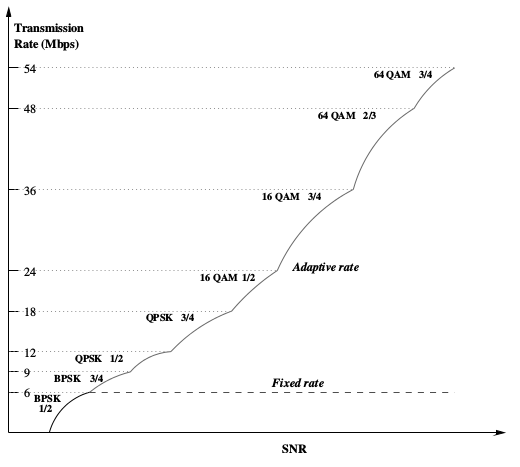
\includegraphics[width=0.6\textwidth]{Adaptive_modulation_and_coding_802_11}
\caption{Адаптивность канала связи в стандарте IEEE 802.11a}
\label{fig:adaptive_modulation_and_coding}
\end{figure}

С помощью адаптивного канального кодирования и модуляции за счет адаптации линии связи может быть обеспечена адаптивная устойчивость к ошибкам. Как показано на рисунке \ref{fig:adaptive_modulation_and_coding}, скорость передачи IEEE 802.11a значительно выше, если применяется адаптация линии связи. По этой причине она широко используется в беспроводных локальных сетях.

Основная концепция адаптации канала довольно проста: настройка параметров передачи (например, количество уровней модуляции, избыточность кодирования) таким образом, чтобы максимизировать использование канала. Тем не менее, необходимо учитывать несколько аспектов при построении адаптивного канала связи.

Для того, чтобы использовать возможности адаптивного кодирования и модуляции на физическом уровне, алгоритм должен быть разработан на уровне MAC, чтобы его рационально использовать. Другими словами, адаптивность канала, как правило, выполняется на уровне MAC. Например, алгоритм управления скоростью должен быть реализован в IEEE 802.11 MAC, чтобы адаптивно выбрать оптимальную скорость передачи в соответствии с канальными условиями. Тем не менее, адаптация линии связи может влиять на разработку протокола MAC. Например, переменное время передачи пакета делает какие-либо механизмы, основанные на подсчете пакетов, бесполезными. Кроме того, когда вычисляется производительность протокола MAC, также необходимо принимать во внимание переменную скорость передачи данных из-за адаптации линии связи.

Другим аспектом является выбор информации о состоянии канала (Channel state information, CSI) и его доступности. CSI представляет собой тип индикатора качества канала. Типичными примерами CSI являются: сигнал-шум (SNR), отношение несущей к помехе (CIR) и BER на физическом уровне, а также частота появления пакетных ошибок (PER) на канальном уровне. Тем не менее, некоторые из них нелегко измерить в беспроводной сети. С другой стороны, единственный тип CSI не может быть достаточной для адаптации линии связи. Например, в среде с частотно-селективными замираниями, алгоритм адаптации линии связи не может принимать SNR или CIR как единственную метрику физического уровня, поскольку в отсутствие других метрик они не отражает реального качества канала.

В некоторых беспроводных сетях адаптация параметров передачи должна быть реализована глубже, чем просто на уровне кодирования или уровней модуляции. Такие параметры как уровень излучаемой мощности, аспекты распространения, возможно, также должны быть адаптированы. С таким большим количеством варьируемых параметров передачи алгоритм адаптации линии связи может быть достаточно сложным. Например, разработка алгоритмов адаптации линии связи для системы MIMO по-прежнему является сложной исследовательской задачей. Кроме того, адаптация канала с таким количеством параметров, как правило, является межуровневой задачей оптимизации между физическим и MAC слоями.

\subsubsection{Направленные антенны}
Для увеличения производительности физического уровня в беспроводном окружении используется направленная связь или устанавливаются многоантенные системы. Нужно отметить, что радиосистема с множеством антенн включает в себя как антенно-фидерную систему, так и обработчик сигнала.

Направленные антенны позволяют осуществлять в беспроводной сети направленные прием и передачу, тем самым обладая несколькими весомыми преимуществами.

\textbf{Лучшая эффективность повторного использования радиочастот.} Поскольку передатчик и приемник являются направленными, повторное использование канала в таком случае не опирается только на пространственное разнесение, что существенно увеличивает эффективность повтого использования радиочастот. Эта особенность позволяет увеличить емкость сети.

\textbf{Меньшая интерференция.} Направленные прием и передача уменьшают число коллизий и интерференцию между различными узлами. Эта особенность увеличивает качество обслуживания и пропускную способность сети.

\textbf{Меньшее энергопотребление для той же емкости сети.} Для аналогичного радиуса связи необходима меньшая мощность излучения.

\textbf{Лучшая безопасность.} Благодаря направленной связи трудно осуществить прослушивание канала, и тем самым растет безопасность сети на физическом уровне.

Направленность антенны может быть достигнута различными способами.

\textbf{Поворачиваемая антенна.} В этом случае одна антенна используется на каждом узле, указывая на определенное направление. Для связи с другими узлами антенну необходимо механически или электически повернуть таким образом, чтобы антенна указывала на нужный курс в необходиое время. Поскольку поворот занимает время, этот вариант может быть нелателен для беспроводной mesh-сети.

\textbf{Переключение антенн.} Каждый узел обладает несколькими антеннами, указывающими на разные направления. Если возникает необходимость передачи данных, узел подключается к антенне, расположенной в нужном секторе. Процесс обладает достаточным быстродействием для нужд беспроводной ячеистой сети. Недостатком данного способа является недостаток гибкости, поскольку направление и радиус покрытия направленной антенны всегда зафиксирован.

\textbf{Формирование луча.} Каждый узел обладает несколькими антеннами. С помощью методик синтеза луча, главный лепесток антенны начинает указывать в нужное направление, в то время как нули диаграммы направленности формируются для нежелательных направлений. С помощью механизмов обработки сигнала, направление главного лепестка может контроллироваться с высокой точностью.

Таким образом, направленность может быть свойством как многоантенной системы, так и передатчика с одной антенной. 

По сравнению с беспроводными сетями без ретрансляции, в беспроводных mesh-сетях применение направленных антенн имеет большие перспективы. Причиной этого является тот факт, что внутри mesh-сети происходит намного более интенсивный обмен данными и выше потребность в радиоресурсе и, таким образом, направленные антенны могут значительно снизить значение данной проблемы. Тем не менее, одновременно с этим увеличивается и сложность управления направленной антенной. Чтобы полностью использовать их преимущества, должны быть перепроектированы протоколы высших уровней. 

\subsubsection{Коллективный прием}
Во множестве случаев многоантенные системы невозомжно применить ввиду недоступности множества антенн. Существует несколько причин, по которым используется единственная антенна на приемопередатчике.
\begin{itemize}
\item Цена и габариты узла. В коммуникационных устройствах, например, карманного формата цена и размер должен оставаться приемлемым. В случае многоантенной системы такой сценарий более труднореализуем.
\item Недостаточное разнесение на одном узле. Для того чтобы построить эффективную многоантенную систему, антенны на одном узле должны располагаться на расстоянии больше половины длины волны. В случае частоты несущей в 5 ГГц минимальное расстояние составляет считанные сантиметры. Но чем частота ниже, тем необходимое расстояние значительнее. Такое габаритное требование не всегда может быть выполнено в мобильном терминале, mesh-клиенте или даже маршрутизаторе.
\end{itemize}

С целью применения разнесения в беспроводных сетях без многоантенных систем было предложено кооперативное разнесение. Идея проста: когда узел А посылает сигнал узлу В, другой узел, например, узел С, который слышит сигнал, также получает его и переотправляет узлу В; как результат, сигнал, полученный узлом В, является суммой сигналов от двух различных, но независимых каналов с затуханием, т. е. пространственное разнесение было достигнуто с помощью кооперативной связи между различными узлами. Таким образом, для достижения разнесения сигнала узлами с единственной антенной каждый узел должен играть две роли: передатчик данных и работа в качестве кооперативного агента для ретрансляции информации другим узлам. 

Из этого базового коцепта получения пользователем кооперативного разнесения следует некоторое количество неоднозначностей:
\begin{itemize}
\item Проблема мощности. Поскоьку одному сигналу необходимо по меньшей мере два различных узла, требуется больше мощности для передачи данных от источника к получателю. С другой стороны, с разнесением излучаемая мощность каждого узла может быть ниже, чем в некооперативном режиме. Таким образом, необходимо разработать механизм установки мощности таким способом, чтобы использовалась минимально возможная мощность для обслуживания кооперативного разнесения пользователей.

\item Проблема скорости передачи данных. В кооперативной связи узлу необходимо передавать данные других узлов, а также отправлять свои собственные данные. Таким образом, его скорость передачи данных снижается. С другой стороны, из-за разнесения, кодовая скорость может быть выше, что увеличивает скорость передачи данных. Таким образом, реальная скорость передачи данных при определенных условиях не снизится.

\item Интерференция. С кооперативным разнесением интерференция также может вырасти из-за передачи одного и того же сигнала по сети более чем один раз. Тем не менее, разнесение может снизить необходимую мощность передатчика, что может скомпенсировать растущую интерференцию.
\end{itemize}

\subsection{Канальный уровень}
\subsubsection{Особенности}
Методы физического уровня для передачи и приема сигнала отвечают за возможность связи между узлами в режиме точка-точка. Тем не менее, этого недостаточно для сетевого общения между несколькими абонентами по нескольким причинам.

Во-первых, необходимо установить интерфейс между протоколами физического и более высокого уровня, для того чтобы интерпретировать битовые потоки и преобразовывать их в пакеты, или наоборот. Во-вторых, механизмы функционирования и алгоритмы необходимы для координации передачи и приема пакетов среди множества узлов с целью повышения производительности сети. Данная функция называется управлением доступа к среде (Media access control, MAC). В-третьих, ошибки все еще могут появляться в битах или пакетах, даже если применяются самые передовые алгоритмы кодирования канала. Это особенно актуально для беспроводных сетей из-за постоянного изменения качества канала связи, возможных помех и многих других факторов. В результате обычно необходим дополнительный контроль ошибок поверх физического уровня.

Основной задачей протокола MAC является координация процесса разделения среды между несколькими пользователями с целью достижения определенных целей производительности. Типичными показателями эффективности являются пропускная способность и параметры QoS: например, задержки, джиттер, коэффициент потери пакетов и т.д.

В зависимости от того как сетевой узел заботится о координации доступа к среде, MAC можно разделить на два основных типа: централизованный MAC и распределенный MAC.

В централизованном варианте протокола MAC весь процесс управляется и координируется центразизующим узлом, все остальные узлы должны обращаться к этому узлу, чтобы получить доступ к сети. Многие беспроводные сети принадлежат к этой категории. Например, сотовые сети, инфраструктурный режим беспроводных локальных сетей, спутниковые сети и т.д. Однако, в беспроводных сетях с множеством ретрансляций предпочтительным является  распределенный вариант MAC, так как сама сеть по сути является распределенной. Если централизованный MAC используется для данного типа сетей, ему не хватает достаточной эффективности в связи с необходимостью поддержания централизованного управления между несколькими узлами. Этот вариант также препятствует масштабируемости протокола MAC. В результате, распределенный MAC крайне необходима для сетей ячеистой топологии. Тем не менее, очевидно, что разработка распределенного MAC является гораздо более сложной задачей, чем разработка централизованного MAC.

Протокол MAC обычно состоит из нескольких основных компонентов.

\begin{enumerate}
\item Обработка пакетов и очередей для передачи и приема. Существует интерфейс между MAC и протоколами верхнего уровня. Когда пакеты поступают из протоколов верхнего уровня, таких как IP, пакеты обрабатываются путем добавления MAC-заголовков и поля контроля ошибок, такого как CRC. Когда существуют требования по безопасности, содержимое пакета должно быть зашифровано в соответствии с определенным алгоритмом шифрования. После завершения обработки пакеты попадают в очередь, и ожидают свободных ресурсов (например, временных интервалов, каналов, кодов и т.д.), чтобы начать передачу. На приемной части весь процесс выполняется в обратном порядке так, чтобы правильно принятые пакеты в слое MAC были отправлены выше.

\item Координация доступа к среде. Этот пункт является ключевым компонентом протокола MAC, который включает в себя множество различных задач, в зависимости от разрабатываемого типа протоколов MAC.

\begin{itemize}
\item Для протокола MAC, основанного на резервировании, ключевой задачей является выделение ресурсов таких как коды, временные интервалы, поднесущие или каналы для пользователей таким образом, что пропускная способность сети максимальна, но их QoS также учитывается. С этой целью следует рассматривать многие другие алгоритмы в необходимости физического уровня, например, управление мощностью, адаптивное кодирование и модуляция и т.д. Кроме того, функции сетевого и транспортного уровней также необходимо учитывать. Например, TDMA MAC может повлиять на производительность TCP при медленном старте вследствие значительных перепадов время прохождения (Round-trip time, RTT) до и после распределения ресурсов. По этой причине может быть важным межуровневое взаимодействие между MAC и протоколами других уровней.

\item Для протокола MAC со случайным доступом, такого как CSMA/CA, ключевым вопросом является выяснение лучшего решения для минимизации коллизий и быстрого восстановления после коллизий в случае, если они все же произойдут. Поскольку не доступно резервирование среды, коллизии становятся серьезным фактором, когда число пользователей увеличивается, и, таким образом, значительно ухудшается пропускная способность. В результате QoS не может быть гарантирована. Тем не менее, MAC протоколы произвольного доступа имеют два основных преимущества. Во-первых, это их простота: нет отдельной сигнализации и схемы резервирования. Во-вторых, совместимость с сетями без установления соединения. Любой же протокол MAC с резервированием всегда сталкивается с проблемой, как осуществить интеграцию с сетью без установления соединения. Например, если используется TDMA MAC, всякий раз, когда начинается TCP сессия, он должен ждать, пока должно быть сделано распределение. Такая задержка не является входит в противоречие с конструкцией TCP, поскольку этот протокол предполагает, что сеть перегружена еще до того как распределение ресурсов завершено. Другим примером является случай, когда видео трафик передается через TDMA MAC в сети Интернет, а MAC не имеет возможности узнать о его пропускной способности и требования QoS. Без такой информации резервирование не может быть сделано правильно, если адаптивная оценка ресурсов и динамическое распределение временных интервалов не осуществляются в интерактивном режиме. Тем не менее, протокол MAC произвольного доступа не имеет какого-либо из этих проблем, так как пакет начинает процесс передачи, как она поступает.
\end{itemize}

\item Адаптивное управление скорости. Физический уровень многих современных беспроводных сетей имеет возможность адаптивного кодирования и модуляции. Для того, чтобы лучше использовать такую возможность, протокол MAC должен учитывать адаптивного управления скоростью для передач пакетов. Вследствие дисперсии скорости передачи, время передачи пакетов также изменяется состояние канала изменяется.

\item Формирование сети и присоединение узлов. Этот компонент фактически является частью управления сетью для протокола MAC. Он заботится о формировании сети и ситуациях, когда узел присоединяется/покидает сеть, что особенно важно в условиях динамической топологии. Без алгоритма формирования сети и присоединения сетевые узлы не в состоянии распознавать друг друга.
\end{enumerate}

Протокол MAC может быть реализован в двух типах архитектуры. В классической архитектура реализации, протокол MAC реализован в программном обеспечении (драйвер MAC), встроенного программного обеспечения и аппаратных средств. Как правило, пакет организации очередей, формирование сети, узел ассоциации, и так далее, выполняются в драйвере. Сроки критически важные функции, например, генерацию временного интервала, процедуры Backoff и т.д., выполняются в прошивке. Фактическая работа в режиме реального времени протокола MAC сделано в аппаратном обеспечении. Например, когда счетчик отсрочки передачи определяется, точный декремент этого счетчика выполняется в аппаратных средствах с целью достижения высокой точности. До сих пор многие компании пытались вытащить больше функций в программном обеспечении на уровне драйверов, так что водитель имеет больше свободы, чтобы контролировать / изменять протокол MAC. Этот тип метода обычно называется реализация «softMAC». Однако, поскольку многие ключевые функции по-прежнему находятся в прошивке, время важной частью протокола MAC трудно изменить. Эта проблема была решена во второй архитектуре реализации, которая называется Software Defined Radio архитектуры (SDR) MAC. В этой новой архитектуре, ни одна прошивка не доступна. Все временные критические функции реализованы на аппаратном уровне, но почти все из них можно управлять или изменения водителем. Таким образом, такая архитектура обеспечивает мощный подход к исследованиям и разработкам новых протоколов MAC.

\subsubsection{Применяемые методы доступа к среде}
Применение существующих протоколов MAC-уровня, в частности протокола множественного доступа с контролем несущей (Carrier Sense Multiple Access, CSMA), ограничено проблемами наложения сигналов, а именно проблемами скрытого и открытого терминала (exposed terminal problem). 

Проблема скрытого терминала возникает, поскольку радиосети, в отличие от других сетей, таких как LAN, не обеспечивают высокую надежность соединения. Таким образом, два узла, которые могут соединиться с третьим, не обязательно могут связаться друг с другом.

Абонент А находится на связи с абонентом B. Узел С также желает взаимодействовать с Узлом В. В соответствии с протоколом CSMA, узел С прослушивает среду, но, поскольку имеется препятствие между узлом A и C, абонент C не в состоянии осуществить передачу данных к А и решает, что среда не занята. Следовательно, С обращается к среде, вызывая коллизии в узле В.

Вторая проблема -- проблема открытого терминала. Пусть узел А передает данные узлу B, а узел С хочет связаться с узлом D. В соответствии с протоколом CSMA абонент С прослушивает среду и обнаруживает, что абонент А передает информацию, и поэтому откладывает доступ к среде. Однако нет никаких причин, по которым узел С не смог бы передавать информацию одновременно с трафиком узла А, поскольку передача узла С не будет мешать приему на узле B из-за большого расстояния между ними. Однако подобная проблема существует, поскольку коллизии происходят в приемнике, в то время как протокол CSMA проверяет состояние среды в передатчике. 

В общем, проблема скрытого терминала снижает ёмкость сети за счет увеличения числа коллизий, в то время как проблема открытого терминала снижает ёмкость в связи с необязательной отсрочкой передачи информации.

Было предложено несколько решений, целью которых являлось снижение вредного действия этих двух проблем. Общей мыслью, отраженной в работах данной тематики, являлась необходимость такого диалога между передающим и приемным узлами, который бы предвосхищал передачу данных; его называют RTS/CTS диалогом.
Узел, готовый передать данные, отправляет пакет управления «запрос на передачу» (Request To Send, RTS), чтобы все устройства, принявшие RTS пакет, отложили доступ к каналу в течение всего срока RTS/CTS диалога. Узел назначения после получения запроса отвечает отправителю коротким управляющим пакетом «готовность к приему» (Clear To Send, CTS). Все узлы, которые принимают пакет CTS, откладывают доступ к каналу на время передачи данных. Прием пакета CTS на передающем узле подтверждает, что диалог RTS/CTS успешно завершен, и узел начинает передачу пакетов пользовательских данных. Хотя диалог RTS/CTS и не исключает проблем скрытого и открытого терминала, он всё же несколько улучшает ситуацию по сравнению с традиционными схемами CSMA. 

\paragraph{Multiple Access Collision Avoidance (MACA)}
В схеме множественного доступа с избежанием коллизий (MACA) для предотвращения коллизий в радиоканале было предложено использовать RTS/CTS диалог. Благодаря его применению в схеме MACA снижена вероятность коллизий пакетов данных, вызванных проблемой скрытых терминалов, но, тем не менее, полностью она не исключена.
 
Как пример такой ситуации -- ошибка приема CTS пакета на некоторых скрытых узлах из-за сеанса связи других узлов. Скрытые узлы без получения какого-либо CTS уведомления в состоянии посылать новые RTS пакеты, в то время как отправитель ответного CTS пакета занят приемом данных от другого узла; как результат -- коллизии данных. Ясно, что для защиты пакетов данных необходимы дополнительные уведомления. 

\paragraph{Схема MACAW (MACA Wireless)}
В протоколе MACAW для пакетной передачи данных применяется обмен сообщениями RTS-CTS-DS-DATA-ACK. К последовательности необходимых в MACA для передачи информации служебных пакетов добавились два новых: DS (Data Sending, пересылка данных) и ACK. После получения пакета CTS абонент посылает DS пакет, сообщающий о начале отправления данных, прежде чем он начинает передавать пакеты пользовательской информации. С помощью данного пакета отправитель уведомляет соседние узлы о том, что диалог RTS/CTS был успешным, и в дальнейшем будет происходить отправка пакетов данных. В свою очередь, сообщение формата ACK было создано для немедленного подтверждения и возможности быстрой повторной передачи испорченных пакетов вместо реализации переотправки на верхних уровнях. 

Для решения проблемы нерационального распределения доступа к общему каналу также был предложен новый алгоритм изменения времени ожидания -- алгоритм многократного увеличения и линейного уменьшения (Multiple Increase and Linear Decrease, MILD). В данном алгоритме на узлах, успешно осуществляющих передачу данных, интервал ожидания уменьшается на один шаг, в случае же неудачной передачи интервал увеличивается в полтора раза. Интервал ожидания также помещается в заголовок передаваемого пакета; таким образом участвующие в процессе передачи узлы могут скопировать его в локальную переменную и использовать. По сравнению с алгоритмом двоичного экспоненциального времени ожидания (Binary Exponential Back-off, BEB) алгоритм MILD обладает более низким разбросом значений интервалов. Дополнительные возможности алгоритма MILD, одной из которых является задание различных интервалов для различных направлений маршрутизации, также повышают справедливость распределения доступа к среде в сети с применением протокола MACAW. 

Недостатком схемы MACAW, унаследованным от схемы MACA, является наличие столкновений пакетов RTS/CTS в сети со скрытыми терминалами, что приводит к ухудшению работы протокола.

\paragraph{Floor Acquisition Multiple Access (FAMA)}
В FAMA каждый готовый к передаче узел должен приобрести канал (<<поверхность>>, floor), прежде чем использовать его для передачи данных. В FAMA для обеспечения приобретения канала и успешной отправки пакетов данных используется как контроль несущей, так и RTS/CTS диалог. Качество работы данного протокола доступа к среде сравнимо с MACA при наличии скрытых терминалов и CSMA в ином случае. Существует несколько модификаций данной технологии: FAMA-NPS (FAMA Non-persistent Packet Sensing, непостоянное прослушивание пакетов FAMA) и FAMA-NCS (FAMA Non-persistent Carrier Sensing, непостоянное прослушивание несущей FAMA). В FAMA-NPS для отсрочки передачи требуется считывание пакетов узлов; протокол FAMA-NCS использует прослушивание несущей, чтобы удержать соседние узлы от передачи во время, когда канал используется для передачи пакетов данных. Длина пакета CTS больше, чем пакета RTS, что поддерживает главенство CTS в ситуации коллизий. Узлы могут прослушивать несущую пакета CTS, когда происходит столкновение между RTS и CTS, и не передавать данные; поэтому пакеты в приемнике защищены.

По итогам исследований было показано, что применение технологии FAMA-NPS в сетях со скрытыми терминалами не вызывает улучшения производительности в отсутствие многократной передачи пакетов CTS. Причина таких результатов -- в возможных столкновениях пакетов как результата работы скрытых терминалов. Протокол FAMA-NCS, путем комбинирования схем контроля несущей и приобретения канала, превосходит CSMA и предыдущие схемы FAMA для многоскачковых сетей. 

С другой стороны существует проблема применения стандарта FAMA-NCS, которая заключается в ложном обнаружении преобладания CTS пакетов. В схеме FAMA-NCS узлу, прослушивающему несущую столкнувшихся пакетов, требуется в ходе передачи данных молчать, даже если коллизии были вызваны пакетами RTS. Поэтому общий канал будет простаивать и использоваться нецелесообразно. Ложное обнаружение преобладания CTS влечет за собой необязательно долгое время простоя среды передачи, что вызывает снижение пропускной способности. 

\paragraph{Dual Busy Tone Multiple Access (DBTMA)}
В случае использования схемы множественного доступа с двойным сигналом занятости (DBTMA) в дополнение к применению пакета RTS задействуются два сигнала занятости, находящие вне полосы частот для передачи данных. Внеполосные тона занятости используются для уведомления соседних узлов о состоянии канала: когда узел готов к передаче, он задействует передающий сигнал занятости и посылает RTS пакет к приемнику. При получении пакета RTS приемник применяет второй сигнал занятости, приемный, и ждет входящего пакета данных. С помощью двух сигналов занятости вероятность коллизий пакетов RTS уменьшается, а производительность сети повышается. 

Схема DBTMA полностью решает проблему скрытого и выставленного терминала. При её применении скрытым терминалам запрещается отправка любых пакетов на протяжении времени получения приемником данных. Это позволяет открытым терминалам инициировать передачу, посылая пакеты RTS. Кроме того, схема позволяет скрытым терминалам отвечать на RTS пакеты, задавая приемный сигнал занятости, и инициировать получение пакетов данных.

\subsection{Сетевой уровень}
Протокол маршрутизации может быть рассмотрен в контексте задачи оптимизации: для любого источника и назначения найти путь маршрутизации, обеспечивающий максимальную производительность, при условии соблюдения ряда ограничений, таких как топология сети и помехи.

Хотя задачи оптимизации варьируются от одного алгоритма маршрутизации к другому, он должен подчиняться принципу оптимальности, то есть если промежуточный узел R находится на оптимальном пути $p(X, Y)$ от узла $X$ в узел $Y$, то оптимальный путь $p(R, Y)$ от $R$ до $Y$ должны быть на том же маршруте $p(X, Y)$. Основываясь на этом принципе, оптимальные пути от всех источников к месту назначения образуют дерево, с корнем в пункте назначения. Следует отметить, что деревья не обязательно являются уникальными, так как существует несколько путей маршрутизации из того же источника, в том же направлении, но ту же самую производительность. В результате маршрутизация эквивалентна процессу обнаружения различных деревьев и использования таких деревьев, для формирования путь маршрутизации для любого источника и назначения.

Тем не менее, в действительности проблема маршрутизации оказывается гораздо более сложным вопросом, особенно когда беспроводная сеть является многоскачковой. Ниже приводится краткое изложение факторов, которые делают маршрутизацию более сложной задачей, чем просто поиск путей маршрутизации на основе деревьев.

Топология сети может быть переменной и непоследовательной. Основные причины этого включают в себя следующие факторы:
\begin{itemize}
\item Связи между узлами могут быть добавляться и пропадать, что особенно верно для беспроводной сети из-за помех, затухания и так далее. Такие изменения могут привести к несогласованному представлению каналов в топологии сети у различных узлов в той же сети.
\item Аналогично связать изменения, топология сети также может быть изменен из-за мобильности узлов или других видов деятельности узлов, таких как соединения или выходе из сети.
\end{itemize}

Метрика маршрутизации не может быть определена просто исходя из топологии сети. Существуют следующие варианты:
\begin{itemize}
\item Метрика маршрутизации больше, чем просто параметр топологии. Например, если считается только количество переходов, выбор пути маршрутизации определяется исключительно топологией сети. По этой причине рассматриваются другие метрики маршрутизации, например, задержка; тогда выбор пути маршрутизации не только связан с топологией сети, но также зависит от помех от узлов, не будучи от выбранных путей маршрутизации. Такие метрики маршрутизации вызывают две сложности: выбор одного пути маршрутизации в сочетании с, что другого пути маршрутизации;  определение маршрутизации путь связан с механизмами распределения ресурсов, включая распределение каналов, управление доступом к среде, управление мощностью, и так далее.
\item Выбор пути маршрутизации должен учитывать распределение трафика в сети для достижения балансировки нагрузки. Тем не менее, распределение трафика также является результатом маршрутизации. Таким образом, балансировка нагрузки и маршрутизация тесно связаны друг с другом. Относительно беспроводных сетей ячеистой топологии эта проблема гораздо сложнее, так как нагрузка трафика звена воздействия нескольких звеньев в диапазоне помех.
\item Там не может быть оптимальным решением для данной задачи маршрутизации. Как было объяснено выше, маршрутизация в сочетании со многими другими функциями, такими как схемы распределения ресурсов. Кроме того, выбор одного пути маршрутизации может зависеть от другого. Учитывая такую сложную задачу оптимизации с возможными ограничениями конфликтов, оптимальное решение может быть недоступна.
\end{itemize}

При маршрутизации рассматривается в рамках оптимизации, обычно формализуется как глобальная или централизованная задача оптимизации. Такая методика не применима к практическим протокола маршрутизации. Таким образом, существует еще один сложный вопрос для маршрутизации: как спроектировать распределенный алгоритм для аппроксимации оптимизации решения глобального алгоритма маршрутизации.

Несмотря на наличие многих протоколов маршрутизации для беспроводных сетей с множеством ретрансляций, особенно для мобильных одноранговых сетей, разработка протоколов маршрутизации остается активным направлением исследований по нескольким причинам.
\begin{itemize}
\item Новые метрики маршрутизации должны быть обнаружены и использованы для повышения производительности протоколов маршрутизации. Наиболее часто используемые метрики до сих пор для протоколов маршрутизации включают счетчик переходов и качество связи. Тем не менее, они далеки от удовлетворения потребности маршрутизации для беспроводных сетей ячеистой топологии, поскольку нахождение оптимального маршрута зависит от различных задач проектирования и сетевых характеристик сети.
\item Для MANET основной проблемой в маршрутизации является высокая мобильность во всех узлах; необходимы сложные процедуры для поддержки такой мобильности. Тем не менее, такие сложности не нужны в mesh-сетях, так как слой маршрутизаторов, как правило, имеет минимальную подвижность. Таким образом, эффективные и легкие протоколы маршрутизации должны быть разработаны для достижения удовлетворительной работы в mesh-сетях.
\item Протоколы маршрутизации для других беспроводных сетей с множеством ретрансляций используют протокол MAC в качестве прозрачного слоя маршрутизации. Тем не менее, необходимо учитывать межуровневое взаимодействие  для того, чтобы улучшить рабочие характеристики протоколов маршрутизации в mesh-сетях.
\end{itemize}

Традиционно сетевые протоколы маршрутизации делятся на проактивные (табличные) и реактивные. В первом случае протоколы непрерывно изучают топологию сети, обмениваясь информацией между сетевыми узлами. Таким образом, когда возникает необходимость в использовании маршрута до пункта назначения, информация о нем может быть получена незамедлительно. 

Первыми протоколами, предложенными для маршрутизации в ad-hoc-сетях, являются проактивные протоколы вектора расстояния, базирующиеся на распределенном алгоритме Беллмана-Форда. Данные протоколы обладают некоторыми проблемами, такими как сходимость (конвергенция) и чрезмерный уровень управляющего трафика; в качестве решения были предложены различные модификации протоколов. Другим подходом, решающим проблему конвергенции, являлось применение протоколов состояния каналов в ad-hoc-среде; как пример -- протокол OLSR (Optimized Link State Routing, оптимизированная маршрутизация состояния каналов).

Иным методом, выбранном некоторыми исследователями, является использование проактивных алгоритмов поиска пути. В таком решении, которое совмещает особенности протоколов вектора расстояния и состояния каналов, каждый узел сети сооружает минимальное ветвящееся дерево (minimal spanning tree), используя информацию минимального ветвящегося дерева о его соседях вместе со стоимостью соединения с ними. Алгоритмы поиска пути позволяют снизить объем служебной информации, уменьшить возможность маршрутных петель и избежать проблему «счета до бесконечности». Пример такого типа маршрутизационных протоколов -- WRP (Wireless Routing Protocol, протокол беспроводной маршрутизации).
 
Главная проблема, сопряженная с применением проактивных протоколов применительно к ad-hoc-сетям, связана с фактом непрерывного изменения топологии сети, поскольку цена поддержания актуальности топологической информации в таком случае может быть высокой. Более того, если активность сети низка, информация об актуальной топологии может практически не использоваться и, таким образом, ограниченные приемопередающие и вычислительные ресурсы, обслуживающие такую сеть, будут использованы неэффективно. 

С другой стороны -- реактивные маршрутизационные протоколы, базирующиеся на диалоге «запрос-ответ». Реактивные протоколы не позволяют непрерывно поддерживать актуальную информацию о топологии сети; напротив, реактивный протокол инициирует процедуру поиска пути к пункту назначения, только когда возникает подобная необходимость,. Подобная процедура включает в себя широковещательную рассылку по сети маршрутных запросов; такие протоколы на практике часто называют протоколами «по требованию» (On-Demand). Примерами реактивных протоколов являются: TORA (Temporally Ordered Routing Algorithm, алгоритм маршрутизации по временному требованию), DSR (Dynamic Source Routing, маршрутизация динамического источника), AODV (Ad hoc On-Demand Distance Vector Routing, маршрутизация вектора расстояния ad-hoc-сетей по требованию). В случае TORA маршрутные запросы используют рассылку для распространения маршрутизационной информации через разновидность направленного ациклического графа, корнем которого является пункт назначения. Протоколы DSR и AODV, с другой стороны, используют одноадресную рассылку чтобы маршрутизировать ответ назад к источнику по обратному пути. В протоколе DSR обратный маршрут содержится в пакете как «накопленный» путь и используется для маршрутизации источника. В AODV информация о пути хранится в узлах, составляющих маршрут, в виде «следующего шага» (перехода на один узел). Хотя реактивные методы могут привести к снижению уровня управляющего трафика по сравнению с проактивными протоколами вектора расстояния или состояния канала, в частности когда активность сети низка и топология быстро изменяется, объем трафика всё еще может быть значительным. Кроме того, задержка, связанная с реактивным открытием маршрутов, может быть также существенной.

Таким образом, обе группы протоколов могут не лучшим образом подходить к высокодинамичному сетевому окружению. Хотя проактивные протоколы в состоянии незамедлительно выдать необходимый маршрут, их работа может занять слишком много сетевых ресурсов в попытке содержать всегда актуальную сетевую топологию. Применение реактивных протоколов, с другой стороны, может снизить объем используемых пользовательских ресурсов, но также может вызвать чрезмерные задержки при составлении маршрутизационных запросов. 

Другим вариантом разрешения проблемы маршрутизации является использование гибридных протоколов, соединяющих в себе некоторые аспекты как активных, так и реактивных. ZRP (Zone Routing Protocol, протокол зонной маршрутизации) -- пример такого гибридного решения. В ZRP каждый узел проактивно поддерживает топологию ближайших соседей, таким образом уменьшая объем трафика, присущий чисто проактивным решениям. Чтобы обнаружить маршруты, находящиеся за пределами ближнего круга, узел начинает широковещательную рассылку запросов для их поиска. Размер зоны ближнего круга -- изменяемый параметр, использование которого позволяет оптимизировать работу протокола в зависимости степени узловой мобильности и активности сети. Применение такого алгоритма позволяет снизить задержки открытия маршрутов, присущие чисто реактивным схемам.

\subsubsection{Протоколы маршрутизации единой области (single-scope)}

Главное преимущество этих протоколов в сравнении с многообластными -- их меньшая сложность: в них отсутствует разделение на дальние и ближние узлы и нет необходимости обслуживать иерархические структуры. Более того, они в общем случае проще в реализации как в случае симуляции, так и на практике. Текущие усилия внутри группы исследования mesh-сетей IETF преимущественно сосредоточены на таких протоколах маршрутизации. 

Тем не менее, неэффективное использование ресурсов может привести к идентичной обработке узлов независимо от их относительного положения. В то же время, например, для узла может отсутствовать необходимость в точной информации относительно маршрутизации дальних узлов. Кроме того, маршрутизация единого пространства может работать всё более неэффективно при увеличении размеров сети, т. е. плохо масштабируется.

Маршрутизационные протоколы единой области подразделяют на реактивные и проактивные. Как было указано выше, главное отличие реактивных протоколов -- отсутствие обновлений таблицы маршрутизации до тех пор, пока не возникает необходимость использования маршрута; таким образом могут быть экономно использованы мощности элементов питания и радиочастотные ресурсы. Тем не менее, когда возникает необходимость передачи данных, источнику требуется сначала запросить и определить маршут, что может привести к маршрутизационным задержкам. Более того, необходим эффективный механизм запроса маршрута, дабы пресечь перегрузку сети пакетами запросов. 

С другой стороны, проактивные протоколы оперируют готовыми маршрутами ко всем узлам. При их использовании исключены задержки маршрутизации или значительный трафик запросов. Недостаток проактивных протоколов заключается в том, что в сети может создаваться лишний служебный трафик для поддержания топологической информации актуальной вне зависимости от необходимости подобных сведений. 

\paragraph{Ad hoc On-Demand Distance Vector Routing (AODV)}
AODV представляет собой реализацию идеи подсчета порядкового номера пункта назначения, реализованную в протоколе DSDV, применительно к протоколам «по требованию».

Каждый узел хранит таблицу маршрутизации узлов на один переход от него, содержащую места назначения, к которым имеется маршрут. Маршрут удаляется, если нет необходимости в его использовании, или же автоматически перезапускается по истечении порогового количества времени. 

Если у источника не имеется маршрута до пункта назначения, генерируется пакет запроса пути (route request, RREQ), использующий поиск расширяющимся кольцом: пакет запроса отправляется ближайшим к отправителю узлам, затем соседям данных узлов, т. е. по мере поиска маршрута начинается отправка пакетов с небольшим значением времени жизни (Time-To-Live, TTL), затем TTL постепенно возрастает, если адресат не был найден. 

RREQ содержит порядковый номер узла назначения, который был использован в последний раз, а также текущий порядковый номер исходного узла. Любой узел, который получает RREQ, обновляет свои записи таблицы следующих переходов по отношению к исходному узлу. Узел, у которого имеется маршрут к месту назначения с более высоким порядковым номером, чем тот, что указан в RREQ, рассылает одноадресный маршрутный ответный пакет (Route Reply, RREP) обратно к источнику. После приема пакета RREP каждый промежуточный узел по маршрутам RREP обновляет свои записи таблицы следующего перехода по отношению к узлу назначения, отбрасывая лишние ответные пакеты и RREP с более низким порядковым номером назначения, чем были ранее. 

Когда промежуточный узел обнаруживает нерабочее соединение на активном маршруте, он передает пакет ошибки маршрута (Route Error, RERR) для своих соседей, которые в свою очередь распространяют RERR пакет по направлению к отправителю через все узлы, использовавшие неисправный маршрут. Источник затем может повторно инициировать построение маршрута, если он по-прежнему необходим.

\paragraph{Dynamic Source Routing (DSR)}
В протоколе динамической маршрутизации (DSR) каждый узел хранит кэш маршрутов, который содержит известные пути до адресатов. Если от источника до получателя нет выстроенного маршрута, он передает пакет запроса пути своим соседям. Любой узел, принимающий запрос маршрута, у которого нет пути до пункта назначения, добавляет свой собственный ID и повторяет широковещательную рассылку пакета. Если же узел, принявший пакет, обладает маршрутом к получателю, то запрос маршрута будет направлен по этому пути. Ответ на запрос, в зависимости от симметричности связей, может быть отправлен или по обратному пути к источнику, или инкапсулирован в запрос узла о поиске маршрута к источнику. 

Если промежуточным узлом обнаруживается нерабочее соединение, он посылает пакет ошибки по направлению к источнику, который, если альтернативные маршруты отсутствуют, может повторно инициировать генерацию маршрута.

\paragraph{Temporally Ordered Routing Algorithm (TORA)}
В TORA маршруты к месту назначения определяются направленным ациклическим графом с корнем в пункте назначения. Каждая соединение в сети считается двунаправленным, но для формирования графа к пункту назначения определяется логическое направление всех соединений путем задания значений высоты (height) двум узлам на концах каждой линии связи. Поскольку текущее время необходимо для вычисления высоты узлов, для применения протокола TORA требуются синхронизированные на всех узлах часы. 

Если у источника нет маршрута к пункту назначения (говоря иначе, источник не имеет исходящих граней в графе), он передает в сеть пакет запроса маршрута (route query packet, QRY), который распространяется через соседей. После получения QRY, узел, у которого имеется маршрут к пункту назначения, генерирует пакет обновления маршрута (update packet, UPD), содержащий его собственную высоту. Получив UPD, каждый узел, который не имеет маршрута к месту назначения обновляет свою высоту, чтобы отразить создание исходящих граней. 

Обслуживание маршрута достигается за счет изменения значений высоты узлов и обмена UPD. Поддерживается обнаружение узлами разделов сети: узел, принимающий отраженное от границы раздела сообщение UPD, в таком случае генерирует пустое сообщение (clear message, CLR), которое затем используется для обновления всех маршрутов в пределах раздела.

TORA также поддерживает и проактивный режим работы, в котором пункт назначения инициирует процесс создания маршрута, посылая пакет, который обрабатывается и направляется соседними узлами.

\paragraph{Destination-Sequenced Distance-Vector Routing (DSDV)}
Протокол DSDV представляет собой улучшение по сравнению с обычным протоколом вектора расстояния Беллмана-Форда. Он устраняет зацикливание маршрутов, увеличивает скорость сходимости, а также снижает долю служебных сообщений в сетевом трафике.

В DSDV каждый узел поддерживает таблицу следующего перехода, т.е. таблицу связей с ближними узлами; содержащейся в ней информацией он обменивается с соседними абонентами. Есть два типа обмена данными таблицы: периодическая широковещательная рассылка полной таблицы и событийно-управляемое дополнение табличной информации. Относительная частота дополнений и полного обновления таблицы определяется мобильностью узла. 

К каждому пакету данных, передаваемому во время широковещательного обновления или дополнения таблицы следующих переходов, узел-источник добавляет порядковый номер. Этот порядковый номер распространяется всеми узлами, получившими соответствующие обновления векторов расстояния, и хранится в записи таблицы следующего перехода этих узлов. Узел после получения новой таблицы следующего перехода от соседнего абонента обновляет свой маршрут до пункта назначения, только если новый порядковый номер больше чем записанный, или если новый номер последовательности такой же, как записанный, но новый маршрут короче. 

\paragraph{Wireless Routing Protocol (WRP)}
Протокол беспроводной маршрутизации (WRP) также обеспечивает рост производительности сети по сравнению с протоколом вектора расстояния Беллмана-Форда. Он сокращает число маршрутов зацикливания и обладает механизмом для обеспечения надежного обмена сообщениями обновления.

%В WRP каждый узел содержит матрицу расстояний, включающую в себя все узлы назначения и всех соседей, с помощью которых возможно его достичь. Для каждой пары сосед -- адресат записывается протяженность маршрута; также отмечается узел‑предшественник (predecessor), то есть предпоследний узел маршрута перед получателем. 

Каждый узел-сосед осуществляет широковещательную рассылку своего текущего оптимального маршрута до выбранного места назначения на событийно-ориентированной поэтапной основе. После передачи ожидаются подтверждения получения ото всех соседних узлов, если от каких-либо соседей они отсутствуют, широковещательная рассылка до них будет сделана повторно. Узел, получив пакеты обновления маршрута от соседа, обновляет свою собственную таблицу маршрутизации при условии согласованности новой информации с данными узла-предшественника, полученной от всех его соседей.

\subsubsection{Протоколы маршрутизации с многими областями (multi-scope)}

Подобные протоколы маршрутизации делят узлы на области в зависимости от их взаимного расположения. В частности, больше вычислительных и энергетических ресурсов тратится на обслуживание топологической информации более близкой и, следовательно, часто используемой части сети, что позитивно влияет на масштабируемость и является главным преимуществом протоколов маршрутизации многих областей.

Их недостатком является относительная сложность по сравнению с протоколами маршрутизации с единой областью видимости: необходимы механизмы различения узлов; кроме того, протоколы, как правило, должны обладать возможностью изменения конфигурации с целью адаптации к изменяющейся топологии сети, вариации сетевого трафика и движению узлов. 

Протоколы данного класса можно разделить на плоские (flat) и иерархические. Основным преимуществом плоских протоколов по сравнению с иерархическими является то, что они не требуют узлов, выполняющих специфические функции: назначение всех узлов идентично, они относительно просты в реализации. 

С другой стороны, иерархические протоколы используют узлы со специализированными функциями, чтобы координировать распространение информации местных соединений; ими в разных случаях, например, являются главы кластеров (cluster head), руководители групп (group leader) или шлюзы. Кроме того, особое положение специализированных узлов позволяет обеспечить прямое управление маршрутизацией между постоянными узлами. Однако динамическое поддержание иерархии может потенциально отнять большую долю энергии источников питания и полосы пропускания, особенно когда сеть очень мобильны. Кроме того, необходимы механизмы избежания перегрузки управляющих узлов и снижения трафика в горячих точках.

\paragraph{Zone Routing Protocol (ZRP)}
В протоколе зонной маршрутизации (ZRP) осуществляется гибридная структура маршрутизации, локально активная и глобально реактивная. Каждый узел проактивно объявляет о состоянии соединений на протяжении фиксированного количество промежуточных точек, называемых радиусом зоны. Объявления обеспечивают каждому устройству актуальный вид своей зоны маршрутизации -- совокупность всех узлов и связей, которые доступны в радиусе зоны. Узлы зоны маршрутизации, которые находятся на расстоянии её радиуса, называются периферийными, они  представляют собой границу зоны маршрутизации и играют важную роль в получении маршрутов на зонной основе. Каждый узел имеет соответствующую зону маршрутизации, зоны соседних узлов перекрываются. 

ZRP использует параметры зоны маршрутизации в целях проведения глобальных маршрутов. Вместо того, чтобы слепо транслировать запросы от узла ко всем соседям, ZRP использует сервис под названием bordercasting («рассылка к границам»), который направляет запрос маршрута от абонента к его периферийным узлам посредством многоадресной рассылки. Для выявления периферийных узлов, которых касается запрос, используются специальные механизмы контроля, которые определяют поступление запроса маршрута и отрезают их от распределения запросов дерева граничной рассылки. Такое решение способствует распространению запроса наружу, далеко от его источника и от покрытых областей сети. 

Зоны маршрутизации также помогают улучшить качество и живучесть обнаруженных маршрутов, делая их более устойчивыми к изменениям топологии сети. После того, как пути были обнаружены, зоны обеспечивают улучшенное, в режиме реального времени, обслуживание маршрута. Ветвление транзитных переходов внутри маршрутизируемой зоны позволяет обходить отказавшие связи. Точно так же могут быть выявлены близкие к оптимальным сегменты маршрута, и трафик может быть перенаправлен вдоль коротких путей.

\paragraph{Optimized Link State Routing (OLSR)} Оптимизированная маршрутизация состояния канала (OLSR) представляет собой протокол состояния канала, в котором информация распространяется с помощью техники широковещательных рассылок.

Ключевым понятием в OLSR является многоточечная ретрансляция (multipoint relay, MPR). MPR-набором узла называется подмножество его соседей, которое охватывает все узлы, размещенные на расстоянии до двух транзитных переходов от источника. Каждый узел получает топологию через периодическую широковещательную рассылку соседями hello-пакетов, которые содержат, в свою очередь, списки их соседей. 

Как и в случае с обычным протоколом состояния канала, информация об обновлении соединений узла распространяется по всей сети. Тем не менее, в OLSR, когда узел отправляет пакет обновления связей, только абоненты в MPR-списке узла участвуют в пересылке пакета (по аналогии с граничной пересылкой радиусом в 1 переход в ZRP).

Кроме того, узел инициирует обновления каналов только относительно тех связей, которые существуют между ним и узлами из его MPR набора. Таким образом, маршруты вычисляются с использованием частичного вида сетевой топологии узла.

\paragraph{Fisheye State Routing (FSR)}
Концепция fisheye («рыбий глаз») основывается на том предположении, что изменения в топологии области сети с увеличением расстояния (в переходах) между источником и сетью оказывают всё меньшее влияние на решения отправителя о продвижении пакетов. Эта зависимость может быть использована в целях уменьшения трафика маршрутизации путем более редкой ретрансляции обновления топологии для отдаленных районов, нежели обновления для близлежащих регионов. Узел может передавать пакет в правильном направлении к месту назначения, учитывая только примерный вид дальних частей сети. По мере продвижения пакета в сторону назначения вид региона получателя становится более точным, обеспечивая более точную пересылку пакетов.

Данный принцип применяется в FSR, адаптации протокола GSR (Global State Routing, маршрутизация глобального состояния). В последнем информация о состоянии канала передается через сеть периодическими обменами таблиц состояния каналов между соседями. В FSR узел обменивается отдельными записями состояния связей с различной периодичностью, в зависимости от расстояния до источника соединения.

\paragraph{Сore-Extraction Distributed Ad hoc Routing (CEDAR)}
В механизме маршрутизации CEDAR используется набор основных узлов (core nodes), составляющих ядро сети, причем по крайней мере один из них находится в пределах одного перехода каждого узла. Узлы, составляющие ядро сети, являются главенствующими по отношению к остальным. Неосновные узлы с помощью периодического обновления получают список идентификаторов своих соседей и основных узлов своих соседей. Информация о состоянии каждого звена распространяется через узлы ядра сети; чем выше пропускная способность линии связи, тем дальше распространяется информация. Каждый основной узел хранит локальную таблицу состояний каналов, содержащую только постоянные ближайшие связи с высокой пропускной способностью.
 
Глобальный поиск маршрут осуществляется реактивно. Основной узел отправителя определяет путь через ядро сети к основному получателя, применяя широковещательную рассылку. Используя свои данные о состоянии канала, основной узел источника вычисляет наиболее короткий и быстрый QoS-допустимый путь с промежуточными узлами к месту назначения. После чего он отправляет запрос о продвижении по маршруту на основной узел промежуточного узла, который затем начинает поиск QoS-допустимых путей по тому же алгоритму. Процесс продолжается до тех пор, пока QoS-допустимый путь не достигнет места назначения, после чего источник начинает пересылку данных.

\paragraph{Zone-based Hierarchical Link State (ZHLS)}
При использовании ZHLS зона покрытия система делится на непересекающиеся физические зоны. Узлы оборудованы геолокационными устройствами, такими как GPS приемники, так что каждый узел может определить свою принадлежность к какой-либо зоне путем сравнения своего физического местоположения с картой. Кроме того, если узлы в пределах зоны по какой-либо причине разделены, создаются логические подзоны, каждая из которых содержит одну из разделенных областей. Каждый узел поддерживает внутризоновую и межзоновую таблицу маршрутизации; внутризоновая таблица маршрутизации позволяет узлу достичь все остальные узлы зоны, межзоновые связи осуществляются через узлы сопряжения (шлюзы) вблизи краев зоны. Шлюзы с помощью широковещательной рассылки информируют всю сеть о статусе виртуальных каналов между зонами. Узел собирает все сообщения шлюзов для формирования межзоновой таблицы маршрутизации. 

Пусть узлу источника необходимо передать данные получателю за пределами зоны отправителя; в таком случае используется запрос по глобальной зоне для определения принадлежности к какой-либо зоне узла назначения. Используя свою межзоновую таблицу маршрутизации, источник посылает запрос ко всем зонам в сети. После получения сообщения запроса, шлюз, зона которого содержит узел назначения, отправляет обратно исходному узлу идентификатор зоны пункта назначения. Затем узел источника начинает посылает пакеты данных с идентификатором зоны получателя и идентификатором самого узла назначения, что указывается в заголовках пакетов. Затем информация пересылается через транзитные узлы получателю в соответствии с внутризоновыми и межзоновыми таблицами маршрутизации.

\paragraph{Landmark Ad hoc Routing (LANMAR)}
В соответствии со схемой ad-hoc-маршрутизации по ориентирам (LANMAR) сеть состоит из заранее определенных логических подсетей, каждая из которых имеет предварительно выбранный ориентир (landmark). Предполагается, что все узлы в подсети двигаются скоординированно, соединение между ними поддерживается с помощью FSR. 

Маршруты к ориентирам и, следовательно, соответствующим подсетям проактивно поддерживаются всеми узлами в сети путем обмена векторами расстояния. Каждый узел имеет бессрочный иерархический адрес, определяющий подсеть, к которой принадлежит абонент. Источник отражает иерархический адрес узла назначения в заголовках пакетов данных. Затем пакеты направляются к ориентиру подсети, к которой принадлежит узел назначения. Когда пакет достигает узла необходимой подсети, пакет пересылается к узлу назначения с помощью таблицы маршрутизации подсети.

\subsubsection{Протоколы географической маршрутизации}

\paragraph{Location-aided routing (LAR)}
В маршрутизации при помощи местоположения (LAR) источник оценивает область места назначения, основываясь на последней известной скорости пункта назначения, и рассылает запрос маршрута только узлам, географически соответствующим данной области. LAR требуется получение географических координат от каждого узла через устройства геопозиционирования (GPS, ГЛОНАСС).

\paragraph{Distance routing effect algorithm for mobility (DREAM)}
В DREAM каждый узел получает свое географическое местоположение с помощью устройств геопозиционирования и периодически передает координаты местоположения на другие узлы в сети. Период передачи местоположения зависит от скорости узла и географического расстояния до узлов, которым информация о местоположении предназначена. 

Источник посылает пакет данных в подмножество своих соседей в направлении пункта назначения. Промежуточные узлы аналогичным образом передают пакет данных к адресату.

\section{РЕШЕНИЕ ОПТИМИЗАЦИОННОЙ ЗАДАЧИ}
\subsection{Классификация методов оптимизации}
Оптимизация -- задача вычисления минимума или максимума целевой функции в некоторой области конечномерного пространства, ограниченной набором линейных и/или нелинейных равенств и/или неравенств.

В процессе проектирования, как правило, ставится задача определения в некотором смысле наилучших значений параметров объектов или их структуры; такая задача называется оптимизационной. Если процесс оптимизации связан с вычислением оптимальных значений параметров при заданной структуре объекта, такая оптимизация называется параметрической. Задача выбора оптимальной структуры является структурной оптимизацией.

Общая запись проблемы оптимизации определяет большое разнообразие классов задач, от которых зависит подбор метода решения. Классификацию задач определяют целевая функция и её допустимая область значений (ограничивается системой неравенств и равенств либо более сложным алгоритмом). Методы оптимизации классифицируются в соответствии с задачами оптимизации: 
\begin{itemize}
\item Локальные методы: сходятся к какому-нибудь локальному экстремуму целевой функции. В случае унимодальной целевой функции, этот экстремум единственен, и будет глобальным максимумом/минимумом;
\item Глобальные методы: имеют дело с целевыми функциями многих экстремумов. При глобальном поиске основной задачей является выявление тенденций глобального поведения целевой функции. 
\end{itemize}

Существующие в настоящее время методы поиска можно разбить на три большие группы: 
\begin{itemize}
\item Детерминированные; 
\item Случайные (стохастические);
\item Комбинированные.
\end{itemize}

По критерию размерности допустимого множества, методы оптимизации делят на методы одномерной оптимизации и методы многомерной оптимизации. 

Задачи оптимизации, в которых целевая функция и ограничения являются линейными функциями, разрешаются так называемыми методами линейного программирования.

По требованиям к гладкости и наличию у целевой функции частных производных, их также можно разделить на следующие: 
\begin{itemize}
\item Прямые методы, требующие только вычислений целевой функции в точках приближений; 
\item Методы первого порядка: требуют вычисления первых частных производных функции; 
\item Методы второго порядка: требуют вычисления вторых частных производных, то есть гессиана целевой функции. 
\end{itemize}

В зависимости от природы множества X задачи математического программирования классифицируются как: 
\begin{itemize}
\item Задачи дискретного программирования (или комбинаторной оптимизации) -- если X конечное или счетное; 
\item Задачи целочисленного программирования -- если X является подмножеством множества целых чисел;
\item Задачи нелинейного программирования, если ограничения или целевая функция содержат нелинейные функции и X является подмножеством конечномерного векторного пространства. 
\end{itemize}

Если же все ограничения и целевая функция содержат лишь линейные функции, то это -- задача линейного программирования. Кроме того, разделами математического программирования являются параметрическое, динамическое и стохастическое программирование. 

\subsection{Элементы теории графов}
Для математического описания инфокоммуникационных сетей принято использовать теорию графов. Теория графов -- раздел дискретной математики, изучающий свойства объектов, называемых графами. В общем смысле граф представляется как множество вершин (узлов), соединенных ребрами. В строгом определении графом называется такая пара множеств G = (V, E), где V - подмножество любого счетного множества, а E -- подмножество VxV. 

Граф -- это упорядоченная пара, для которой выполнены следующие условия: 
непустое множество вершин (узлов); 
множество пар (в случае неориентированного графа -- неупорядоченных) вершин, называемых ребрами. Вершины и ребра графа называются также элементами графа, число вершин в графе -- порядком, число ребер -- размером графа.

Соединенные некоторым ребром вершины называются концевыми (инцидентными) вершинами (или просто концами) этого ребра. Две концевые вершины одного и того же ребра называются соседними. Два ребра называются смежными, если они имеют общую концевую вершину. 

Степенью вершины называют количество инцидентных ей ребер (при этом петли считают дважды). Вершина называется изолированной, если она не является концом ни для одного ребра; висячей (или листом), если она является концом ровно одного ребра. 

Ориентированный граф -- граф, ребрам которого присвоено направление. Направленные ребра именуются также дугами. 

Орграф D = (V, E) есть множество E упорядоченных пар вершин. 

Дуга (u, v) инцидентна вершинам u и v. При этом говорят, что u -- начальная вершина дуги, а v -- конечная вершина. 

Орграф, полученный из простого графа ориентацией ребер, называется направленным. В отличие от последнего, в произвольном простом орграфе две вершины могут соединяться двумя разнонаправленными дугами.

Маршрутом в орграфе называют чередующуюся последовательность вершин и дуг, от узла-отправителя к получателю (вершины могут повторяться). Длина маршрута -- количество дуг в нем.

Путь есть маршрут в орграфе без повторяющихся дуг, простой путь -- без повторяющихся вершин. Если существует путь из одной вершины в другую, то вторая вершина достижима из первой. 

Орграф называют сильно связным, или просто сильным, если все его вершины взаимно достижимы; односторонне связный, или просто односторонний если для любых двух вершин, по крайней мере одна достижима из другой; слабо связный, или просто слабый, если при игнорировании направления дуг получается связный (мульти)граф. Максимальный сильный подграф называется сильной компонентой; односторонняя компонента и слабая компонента определяются аналогично.

\subsection{Формирование математической модели}
Как уже было отмечено выше, в числе проблем, с которыми так или иначе приходится сталкиваться при работе с сетями ячеистой топологии, состоит и проблема рационального использования сетевых ресурсов при их ограниченности; в случае, например, мобильных ad-hoc-сетей (MANET) возможность перемещения абонентов вызывает энергетические и вычислительные ограничения (так как пользовательские устройства должны иметь невысокий вес и длительное время автономной работы); по правовым и схемотехническим (конструктивным) причинам существуют пределы и для радиочастотных диапазонов. Рассмотрим задачу оптимизации работы сети при ограниченности полосы частот, используемой оборудованием. 

Пусть имеется некоторое число абонентских устройств, составляющих сеть и расположенных друг от друга на различном расстоянии. Каждое из них излучает сигнал некоторой полосы частот, не пересекающейся с остальными передатчиками, с определенной мощностью; уровень излучаемого сигнала зависит от расстояния между узлами. 

Приемопередатчик обменивается данными с остальными абонентами, интенсивность обмена варьируется от узла к узлу сети; могут существовать узлы, приемопередача для которых отсутствует. Данные могут передаваться по одному, двум или более маршрутам от отправителя к получателю. Необходимо определить полосы частот передаваемого сигнала для каждого пользователя по отношению к остальным в зависимости от необходимой пропускной способности каналов, а также оптимальные маршруты для минимизации суммарной задержки передачи данных в сети. 

Иными словами, необходимо определить минимальное значение функции суммарных задержек при заданных параметрах величины сигнала и расстояния между абонентами, а также получить полосы частот и интенсивности потоков для всех маршрутов, при которых данный минимум достигается. 

Для решения задачи следует воспользоваться методами теории графов. В таком случае возможно представить сеть в качестве графа, удовлетворяющего аппроксимации Клейнрока и теореме Джексона, каждая вершина которого будет представлять абонента с необходимыми параметрами, а вес ребер будет отражать отдаленность узлов друг от друга. 

С помощью данного подхода мы получим полный взвешенный орграф с \textit{N} вершин (то есть сеть, в которой присутствует \textit{N} абонентов)~-- граф, каждая пара вершин \textit{i}, \textit{j} ($0 \leq i \leq N, 0 \leq j \leq N$) которого соединена двумя направленными ребрами и имеет вес, зависящий от $R_{i, j}=R_{j, i}$~-- расстояния между узлами. Каждый узел обладает следующими параметрами:

\begin{itemize}
	\item Месторасположение ($x_i$, $y_i$) в прямоугольной системе координат; расстояние $R_{i, j}$ между узлами \textit{i} и \textit{j} определяется по теореме Пифагора;
	\item Мощность передатчика $P_i$;
	\item Полоса частот $\Delta f_i$, задействованная передатчиком ($0 \leq  \sum\limits_{i=1}^N \Delta f_i \leq F$, где \textit{F}~-- рабочая полоса частот всей беспроводной сети);
	\item Вектор пропускной способности $D_i$, каждый элемент которого характеризует требуемую для связи пропускную способность между узлом-отправителем \textit{i} и узлом получателем. Построчно записав все вектора $D_i$ получим матрицу пропускной способности \textit{D};
	\item Пороговая мощность приема $P_{min}$, ниже которой устойчивый прием, ввиду низкого отношения сигнал-шум, невозможен.
\end{itemize}

От каждого абонента до остальных существуют маршруты $\lambda_{i,j}^{m,n,k}$, где \textit{m}~-- номер узла-источника, \textit{n}~-- номер узла-приемника, $m \neq n$, \textit{k}~-- номер маршрута между узлами \textit{m} и \textit{n}; \textit{i}, \textit{j}~-- индексы ребра, направленного от абонента с номером \textit{i} к абоненту с номером \textit{j}. В таком случае суммарный поток через ребро с индексом \textit{i}, \textit{j} будет определен следующим образом:
\begin{equation}
\Lambda_{i,j} = \sum\limits_{m=1}^N\sum\limits_{n=1}^N\sum\limits_{k=1}^K\lambda_{i,j}^{m,n,k} ,
\end{equation}

где \textit{K}~-- число маршрутов между узлами \textit{m} и \textit{n}.

Очевидно, что суммарная скорость передачи данных всех маршрутов, пролегающих через ребро, должна быть меньше пропускной способности канала:
\begin{equation}
\label{eq:mu_greater_lambda}
\mu_{i,j} > \Lambda_{i,j}
\end{equation}

Кроме того, существуют требования по обеспечению пропускной способности между абонентами:
\begin{equation}
\label{eq:lambda_equals_datarate}
\Lambda_{m,n} = \sum\limits_{k=1}^K\lambda_{i,j}^{m,n,k} = D_{m,n}
\end{equation}

Поскольку, в соответствии с аппроксимацией Клейнрока, все информационные потоки можно считать Пуассоновскими, для определения времени задержки для каждого ребра применима формула:
\begin{equation}
\bar{T} = \dfrac{\dfrac{1}{\mu}}{1-\dfrac{\lambda}{\mu}},
\end{equation}

где $\mu$~-- интенсивность обслуживания заявок; $\lambda$~-- интенсивность поступления заявок. Оба параметра измеряются в бит/с.

Максимально возможную интенсивность обслуживания заявок определим по теореме Шеннона-Хартли:
\begin{equation}
\mu_{i,j} = \Delta f_{i,j} \cdot \log_2\left(1 + \dfrac{P_{i,j_{\text{с}}}}{P_{\text{ш}}}\right),
\end{equation}

где $\mu_{i,j}$~-- интенсивность обслуживания заявок между передатчиком \textit{i} и приемником \textit{j}; $\Delta f_{i,j}$~-- используемый при передаче по каналу $i,j$ частотный диапазон ($\sum\limits_{j=1}^N \Delta f_{i,j} = \Delta f_{i}; i \neq j $); $P_{\text{ш}}$~-- мощность теплового шума; $P_{i,j_{\text{с}}}$~-- мощность сигнала в точке приема.

Мощность сигнала в точке приема, в свою очередь, в идеальных условиях связана с расстоянием через формулу передачи Фрииса:
\begin{equation}
\label{eq:friis}
P_{i,j_{\text{с}}} = P_i G_{\textit{пер}} G_{\textit{пр}} \left(\dfrac{c\slash f}{4 \pi R_{i,j}}\right)^2,
\end{equation}

где $G_{\textit{пер}}$~-- коэффициент усиления передающей антенны; $G_{\textit{пр}}$~-- коэффициент усиления приемной антенны; $c\slash f$~-- длина волны несущей.

Для решения задачи минимизации суммарного времени задержки, распределения информационных потоков и радиочастотного диапазона также необходимо учесть, что ограничением будет являться неотрицательность частотных, скоростных характеристик:
\begin{equation}
\label{eq:constraints}
\Delta f_{i,j} \geq 0; \lambda_{i,j}^{m,n,k} \geq 0;  \mu_{i,j} \geq 0 
\end{equation}

Целевая функция, как сумма временных задержек при передаче данных между узлами, также должна быть неотрицательна, как и каждое из ее слагаемых. Суммируя вышесказанное, получим следующую целевую функцию с системой ограничений (\ref{eq:mu_greater_lambda}), (\ref{eq:lambda_equals_datarate}), (\ref{eq:constraints}):

\begin{multline}
F = \sum\limits_{i=1}^N \sum\limits_{j=1}^N \bar{T}(\Lambda_{i,j}, \Delta f_{i,j}) = \\ = \sum\limits_{i=1}^N \sum\limits_{j=1}^N \dfrac{\dfrac{1}{\Delta f_{i,j} \cdot \log_2\left(1 + \dfrac{P_i G_{\textit{пер}} G_{\textit{пр}} \left(\dfrac{c\slash f}{4 \pi R_{i,j}}\right)^2}{P_{\text{ш}}}\right)}}{1-\dfrac{\lambda}{\Delta f_{i,j} \cdot \log_2\left(1 + \dfrac{P_i G_{\textit{пер}} G_{\textit{пр}} \left(\dfrac{c\slash f}{4 \pi R_{i,j}}\right)^2}{P_{\text{ш}}}\right)}} \geq 0
\end{multline}

\subsection{Получение численного решения}
Особенность задачи состоит в том, что регулирование параметров качества обслуживания (в нашем случае задержки при передаче данных) в беспроводной сети как сети с общей средой передачи может осуществляться несколькими способами: перераспределением трафика между существующими маршрутами, либо изменением ширины радиоканала между радиоприемником и передатчиком, причем нахождение оптимума должно включать одновременное рассмотрение как первого способа, так и второго.

По данной причине целевое решение получим в виде вектора, первая часть переменных которого отвечает за поток данных, протекающий через каждый из маршрутов, а вторая~-- частоты, обозначающие полосу частот для каждого из каналов. 
\begin{equation}
X_{\text{опт}} = \begin{pmatrix} \lambda^{1,2,1} &\ldots & \lambda^{N,N-1,K} & \Delta f_{1,2} & \ldots & \Delta f_{N,N-1}\end{pmatrix}
\end{equation}

Первая часть ограничений является следствием (\ref{eq:mu_greater_lambda}) и (\ref{eq:constraints}): сумма потоков данных, протекающих через канал (\textit{i}, \textit{j}), должна быть меньше, нежели пропускная способность канала. Или, иначе говоря, разность суммарного трафика через ребро и пропускной способности канала должна быть отрицательной:
\begin{equation}
\label{eq:restrictions_first}
0 \cdot \lambda^{1,2,1} + \ldots + \lambda_{i,j}^{m,n,k} + \ldots - 0 \cdot \Delta f_{1,2} - \ldots - \log_2\left(1 + \dfrac{P_{i,j_{\text{с}}}}{P_{\text{ш}}}\right) \cdot \Delta f_{i,j} - \ldots < 0
\end{equation}

В ходе решения ограничения (\ref{eq:restrictions_first}) формализуются на языке программирования высокого уровня Python следующим образом:

\listingcaption{Формирование ограничений пропускной способности}
\vspace{0.7\baselineskip}
{\singlespacing
\begin{minted}[breaklines,linenos,fontsize=\small]{python}
for transmitter in range(NODES_NUMBER):
  for receiver in range(NODES_NUMBER):
    if routes_through_links[transmitter][receiver]:
      A_line = []
      for starting_node in range(NODES_NUMBER):
        for end_node in range(NODES_NUMBER):
          for route in nodes_routes[starting_node][end_node]:
            if (starting_node, end_node, nodes_routes[starting_node][end_node].
            index(route)) in routes_through_links[transmitter] [receiver]:
              A_line.append(1)
            else:
              A_line.append(0)
      if A_line:
        for tx in range(0, NODES_NUMBER):
          for rx in range(0, NODES_NUMBER):
            if tx != rx:
              if transmitter == tx and receiver == rx:
                A_line.append(-math.log(1 + received_power[tx][rx] / NOISE_POWER,2) * max_load)
              else:
                A_line.append(0)
        A_ub.append(A_line)
        b_ub.append(0)
\end{minted}
}

Вторая часть ограничений происходит из выражения (\ref{eq:lambda_equals_datarate}):
\begin{equation}
0 \cdot \lambda^{1,2,1} + \ldots + \lambda^{m,n,1} + \ldots + \lambda^{m,n,k} + \ldots + 0 \cdot \Delta f_{1,2} - \ldots - 0 \cdot \Delta f_{i,j} = D_{i,j}
\end{equation}

\listingcaption{Формирование требований обеспечения скорости передачи}
{\singlespacing
\begin{minted}[breaklines,linenos,fontsize=\small]{python}
for starting_node in range(NODES_NUMBER):
  for end_node in range(NODES_NUMBER):
    A_line = []
    if datarates_matrix[starting_node][end_node]:
      for first_node in range(NODES_NUMBER):
        for last_node in range(NODES_NUMBER):
          for route in nodes_routes[first_node][last_node]:
            if starting_node == first_node and end_node == last_node:
              A_line.append(1)
            else:
              A_line.append(0)
      A_line += [0 for tx in range(NODES_NUMBER) for rx in range(NODES_NUMBER) if tx != rx]
      A_eq.append(A_line)
      b_eq.append(datarates_matrix[starting_node] [end_node])
\end{minted}
}

Третья часть ограничений относится к частотам и частотному планированию; сумма группы каналов, входящих в одну частотную область, должна укладываться в частотный диапазон, выделенный на всю сеть:
\begin{equation}
0 \cdot \lambda^{1,2,1} + \ldots + 0 \cdot \lambda^{N,N-1,K} + \Delta f_{i,j} + \cdots + \Delta f_{i,j} \leq F,
\end{equation}

\listingcaption{Формирование частотного плана}
{\singlespacing
\begin{minted}[breaklines,linenos,fontsize=\small]{python}
for dependent_links_set in dependent_links:
  A_line = [0] * total_routes_number
  for transmitter in range(NODES_NUMBER):
    for receiver in range(NODES_NUMBER):
      if transmitter != receiver:
        if (transmitter, receiver) in dependent_links_set:
          A_line.append(1)
        else:
          A_line.append(0)
  A_ub.append(A_line)
  b_ub.append(FREQUENCY_BANDWIDTH)
\end{minted}
}

Количество уравнений при этом будет определяться количеством частотно-независимых областей сети. 

Полный листинг программы оптимизации приведен в приложении А.

Поиск решения будет осуществляться в два этапа: поиск опорного решения и его последующая оптимизация. Для поиска решения, удовлетворяющего всем условиям, воспользуемся симплекс-методом, применяемым в случае оптимизационных задач при линейной системе ограничений. Значения коэффициентов при целевой функции не важны; в данном случае важны лишь значения переменных, удовлетворяющие системе ограничений. Следует заметить, что такой подход в том числе решает вопрос не только определения параметров опорного решения, но также его наличия либо отсутствия~-- в последнем случае из системы уравнений просто не будут выведены вспомогательные переменные, преобразующие неравенства системы в равенства. 

Из-за нелинейности целевой функции оптимизация была проведена с помощью последовательного квадратичного программирования средствами SciPy~-- библиотеки для научных и инженерных расчетов  для языка программирования Python.

\section{ПРИМЕР РЕШЕНИЯ}
Пусть задана сеть из пяти узлов, расположенных на площадке $5\times5$ км. Каждый узел обладает следующими характеристиками:
\begin{itemize}
	\item Координаты ($x_i$, $y_i$)~-- указаны в таблице ниже:
	
	\begin{table}[h]
	Таблица 1 -- Координаты узлов сети \\
	\centering
	\begin{tabular}{|c|c|}
	\hline
	 Порядковый номер узла & Координаты ($x_i$, $y_i$)\\ \hline
	 1 & (4900, 4500) \\ \hline
	 2 & (2900, 240) \\ \hline
	 3 & (4900, 200) \\ \hline
	 4 & (3600, 2400) \\ \hline
	 5 & (3800, 1700) \\ \hline
	\end{tabular}
	\end{table}
	\item Мощность передатчика $P_i$ = 0,1 Вт;
	\item Необходимая скорость передачи данных до каждого узла~-- 1 Мбит/с ($10^6$ бит/с);
	\item Пороговая мощность приема $P_{min}$ = $10^{-12}$ Вт, что соответствует чувствительности среднестатистического современного бытового приемника (--90 дБ по уровню 1 мВт).
	\item Частотный диапазон, выделенный для построения сети, составляет 20 МГц. Частота несущей~-- 2.41 ГГц. 
\end{itemize}

Сначала необходимо определить для каждого передатчика, с какими из присутствующих в сети узлов возможно установление соединения. С этой целью найдем матрицу смежности для графа. Зная координаты передатчика и приемника, найдем расстояние между ними, затем при помощи формулы передачи Фрииса (\ref{eq:friis}) определим мощность принимаемого сигнала, после чего, сравнив ее с пороговой мощностью приема, сделаем вывод о наличии/отсутствии связи. Расчет приводится для изотропных антенн ($G_{\textit{пер}} = G_{\textit{пр}} = 1$). 

В формуле (13) приведена матрица приемных мощностей $P_\textit{пр}$ и матрица смежности \textit{A}.

\begin{equation}
P_\textit{пр} = 
\begin{pmatrix}
0 & 4.54 \cdot 10^{-13} & 5.4 \cdot 10^{-13} & 1.69 \cdot 10^{-12} & 1.15 \cdot 10^{-12} \\
4.54 \cdot 10^{-13} & 0 & 2.57 \cdot 10^{-12} & 1.89 \cdot 10^{-12} & 3.22 \cdot 10^{-12} \\
5.4 \cdot 10^{-13} & 2.57 \cdot 10^{-12} & 0 & 1.5 \cdot 10^{-12} & 2.88 \cdot 10^{-12} \\
1.69 \cdot 10^{-12} & 1.89 \cdot 10^{-12} & 1.5 \cdot 10^{-12} & 0 & 1.84 \cdot 10^{-11} \\
1.15 \cdot 10^{-12} & 3.22 \cdot 10^{-12} & 2.88 \cdot 10^{-12} & 1.84 \cdot 10^{-11} & 0 \\
\end{pmatrix}
\end{equation}
\begin{equation}
A = 
\begin{pmatrix}
0 & 0 & 0 & 1 & 1 \\
0 & 0 & 1 & 1 & 1 \\
0 & 1 & 0 & 1 & 1 \\
1 & 1 & 1 & 0 & 1 \\
1 & 1 & 1 & 1 & 0 \\
\end{pmatrix}
\end{equation}

По матрице смежности А определим, какое количество маршрутов существует между каждым передатчиком и приемником, и какие транзитные узлы пролегают между ними. Из-за значительного количества маршрутов привести сводную таблицу ниже не представляется возможным; общее же число маршрутов для данной топологии~-- 146.

Всего для построения опорного решения суммарно получим 33 линейных уравнения c 162 неизвестными. 

В результате вычислений по вышеописанной методике был получен опорный план, определяющий скорости передачи данных и пропускные способности по каждому из каналов:
% Все, что описано строчкой выше - пропускная способность и СПД
\begin{equation}
\Lambda_{\text{нач}} = 
\begin{pmatrix}
0 & 0 & 0 & 8 \cdot 10^{6} & 6 \cdot 10^{6} \\
0 & 0 & 7 \cdot 10^{6} & 2 \cdot 10^{6} & 3 \cdot 10^{6} \\
0 & 5 \cdot 10^{6} & 0 & 5 \cdot 10^{6} & 2 \cdot 10^{6} \\
8 \cdot 10^{6} & 3 \cdot 10^{6} & 4 \cdot 10^{6} & 0 & 1 \cdot 10^{6} \\
6 \cdot 10^{6} & 4 \cdot 10^{6} & 1 \cdot 10^{6} & 1 \cdot 10^{6} & 0 \\
\end{pmatrix}
\end{equation}
\begin{equation}
\mu_{\text{нач}} = 
\begin{pmatrix}
0 & 0 & 0 & 8008008 & 6006006 \\
0 & 0 & 7007007 & 2002002 & 3003003 \\
0 & 5005005 & 0 & 5005005 & 2002002 \\
8008008 & 3003003 & 4004004 & 0 & 1001001 \\
6006006 & 4004004 & 1001001 & 1001001 & 0 \\
\end{pmatrix}
\end{equation}

Данным $\mu_{\text{нач}}$ и $\Lambda_{\text{нач}}$ соответствует значение целевой функции:
\begin{equation}
F_{\text{нач}}(\mu_{\text{нач}}, \Lambda_{\text{нач}}) = 15987.0194199
\end{equation}

\begin{figure}[h]
\centering
    \begin{subfigure}{0.49\textwidth}
        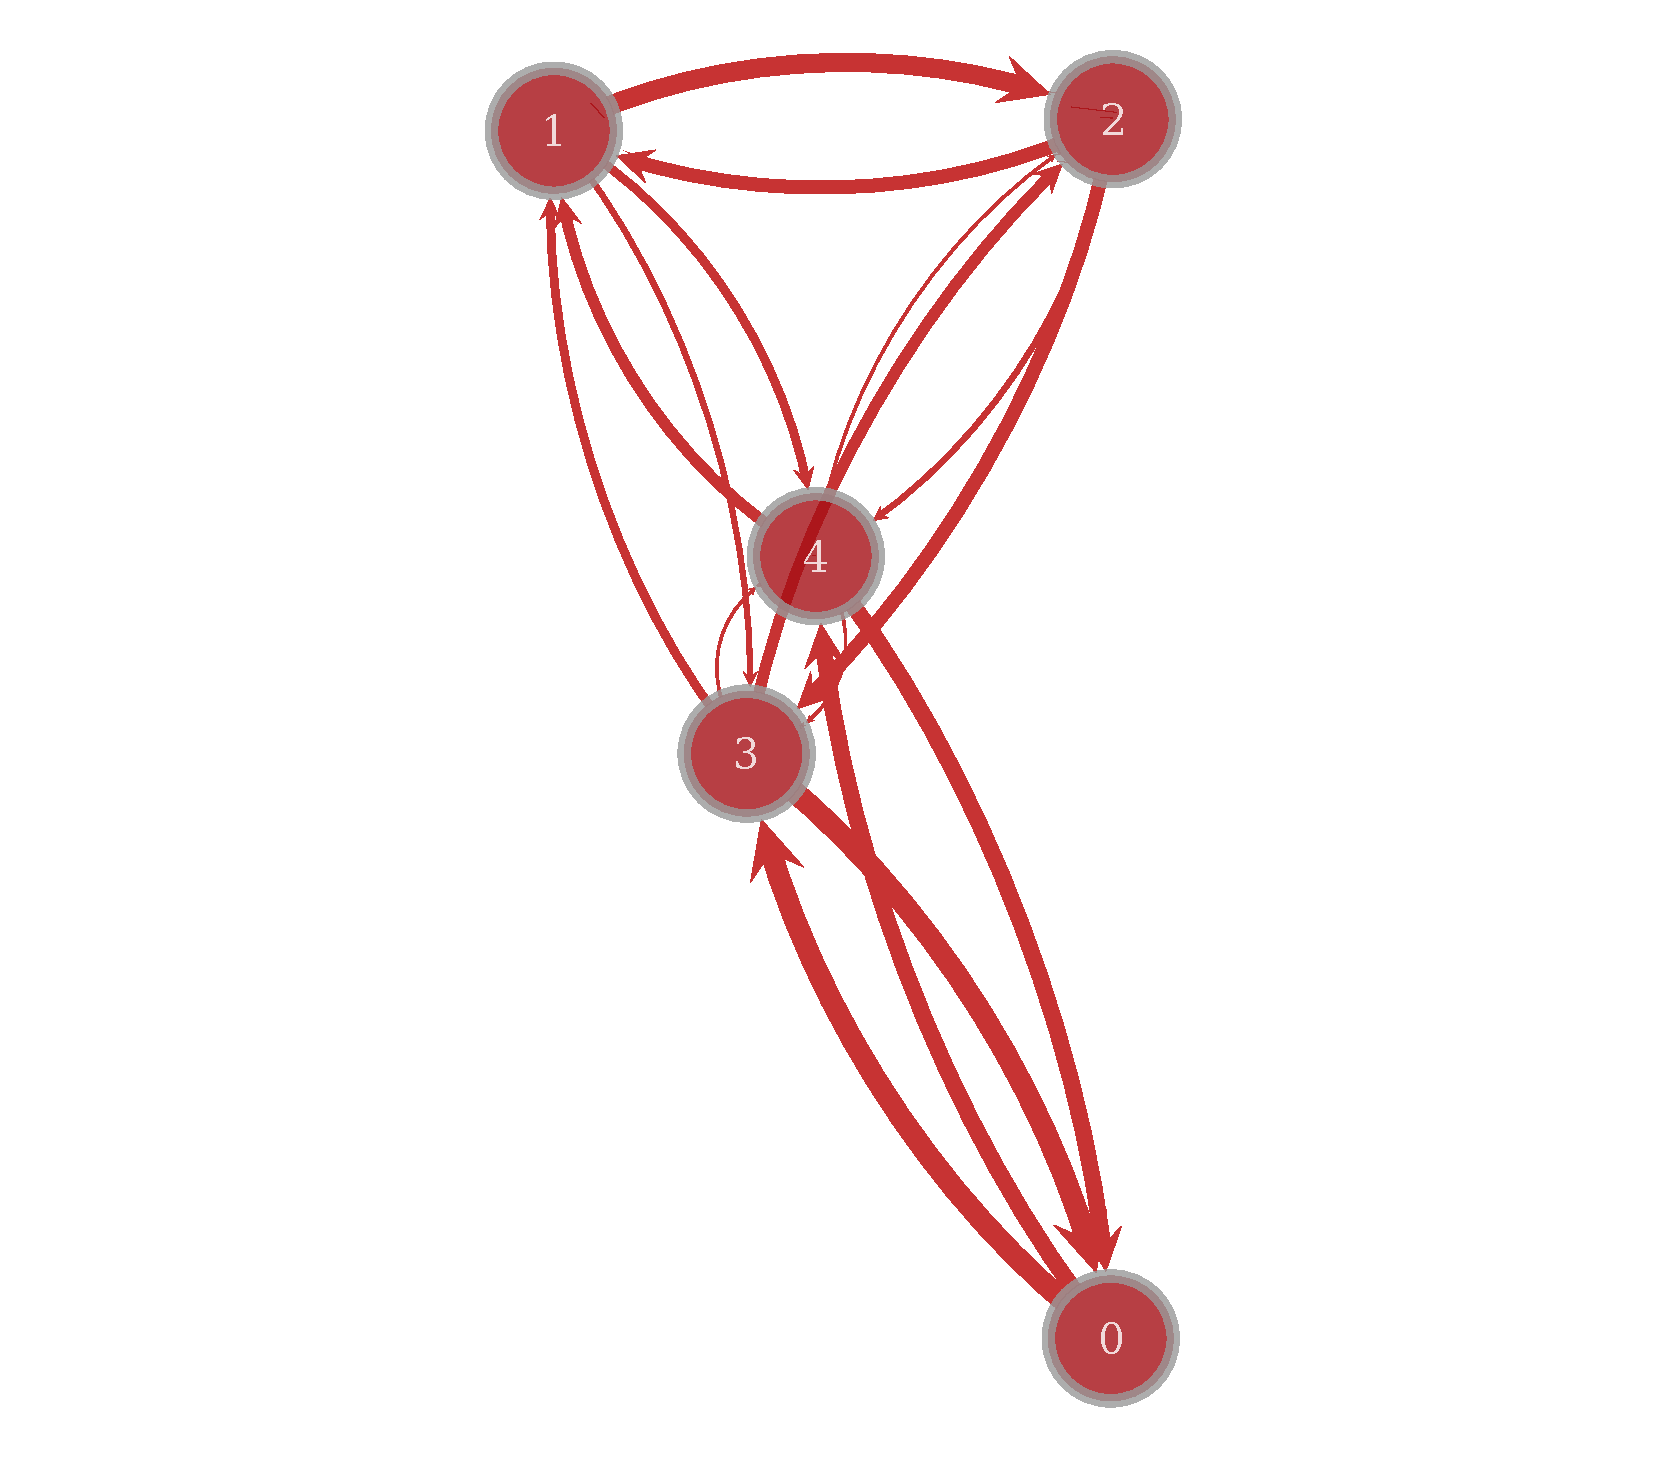
\includegraphics[width=\textwidth]{initial_mu}
        \caption{Сетевой трафик}
        \label{fig:initial_mu}
    \end{subfigure}
    \begin{subfigure}{0.49\textwidth}
        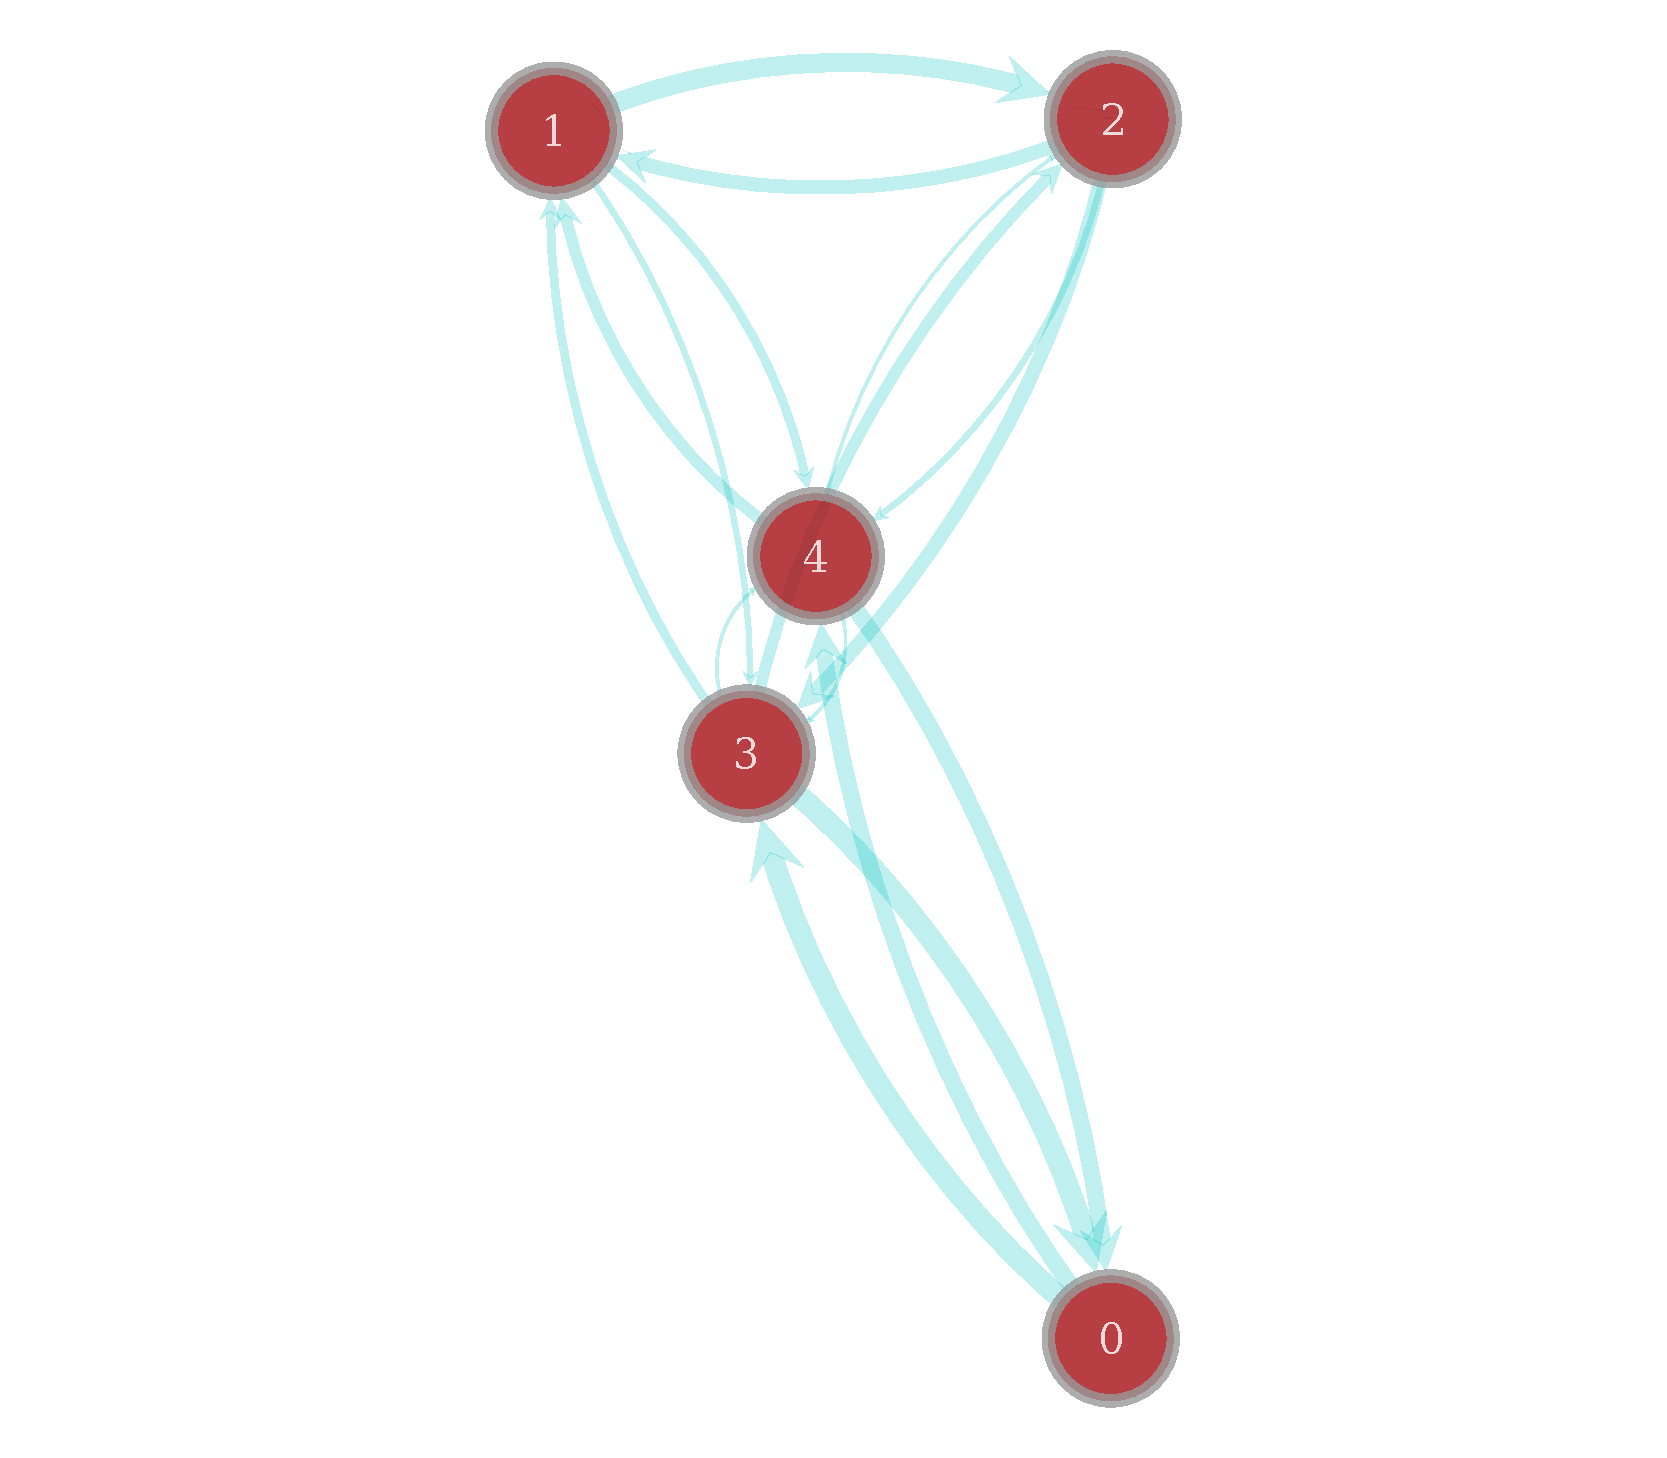
\includegraphics[width=\textwidth]{initial_lambda}
        \caption{Емкость каналов связи}
        \label{fig:initial_lambda}
    \end{subfigure}
    \caption{Визуализация опорного решения}\label{fig:initial_solution}
\end{figure}

С помощью последовательного квадратичного программирования целевая функция затем была оптимизирована. Получены следующие пропускные способности и скорости передачи данных по каналам связи:
\begin{equation}
\Lambda_{\text{опт}} = 
\begin{pmatrix}
0 & 0 & 0 & 5946828 & 4064385.2 \\ 
0 & 0 & 4973011.1 & 1535997.4 & 1860591.1 \\ 
0 & 2904753.9 & 0 & 4426369.6 & 1020489.5 \\
6234577.5 & 2405201.8 & 3074302.6 & 0 & 1381019.2 \\ 
3776635.7 & 3059643.8 & 304299.3 & 1185906.1 & 0 \\
\end{pmatrix}
\end{equation}
\begin{equation}
\mu_{\text{опт}} = 
\begin{pmatrix}
0 & 0.0 & 0.0 & 11650190 & 9770303\\ 
0.0 & 0 & 12340662 & 16561260 & 16445313\\
0.0 & 12371381 & 0 & 10377969 & 20280460\\
11685991 & 13054022 & 10667930 & 0 & 67045227\\ 
9763645 & 14290214 & 33341686 & 67041824 & 0\\
\end{pmatrix}
\end{equation}
% СПД и пропускная способность, соответствующая оптимизированной.

При этом значение целевой функции:
\begin{equation}
F_{\text{опт}}(\mu_{\text{опт}}, \Lambda_{\text{опт}}) = 6.48920601529
\end{equation}

\begin{figure}[h]
\centering
    \begin{subfigure}{0.49\textwidth}
        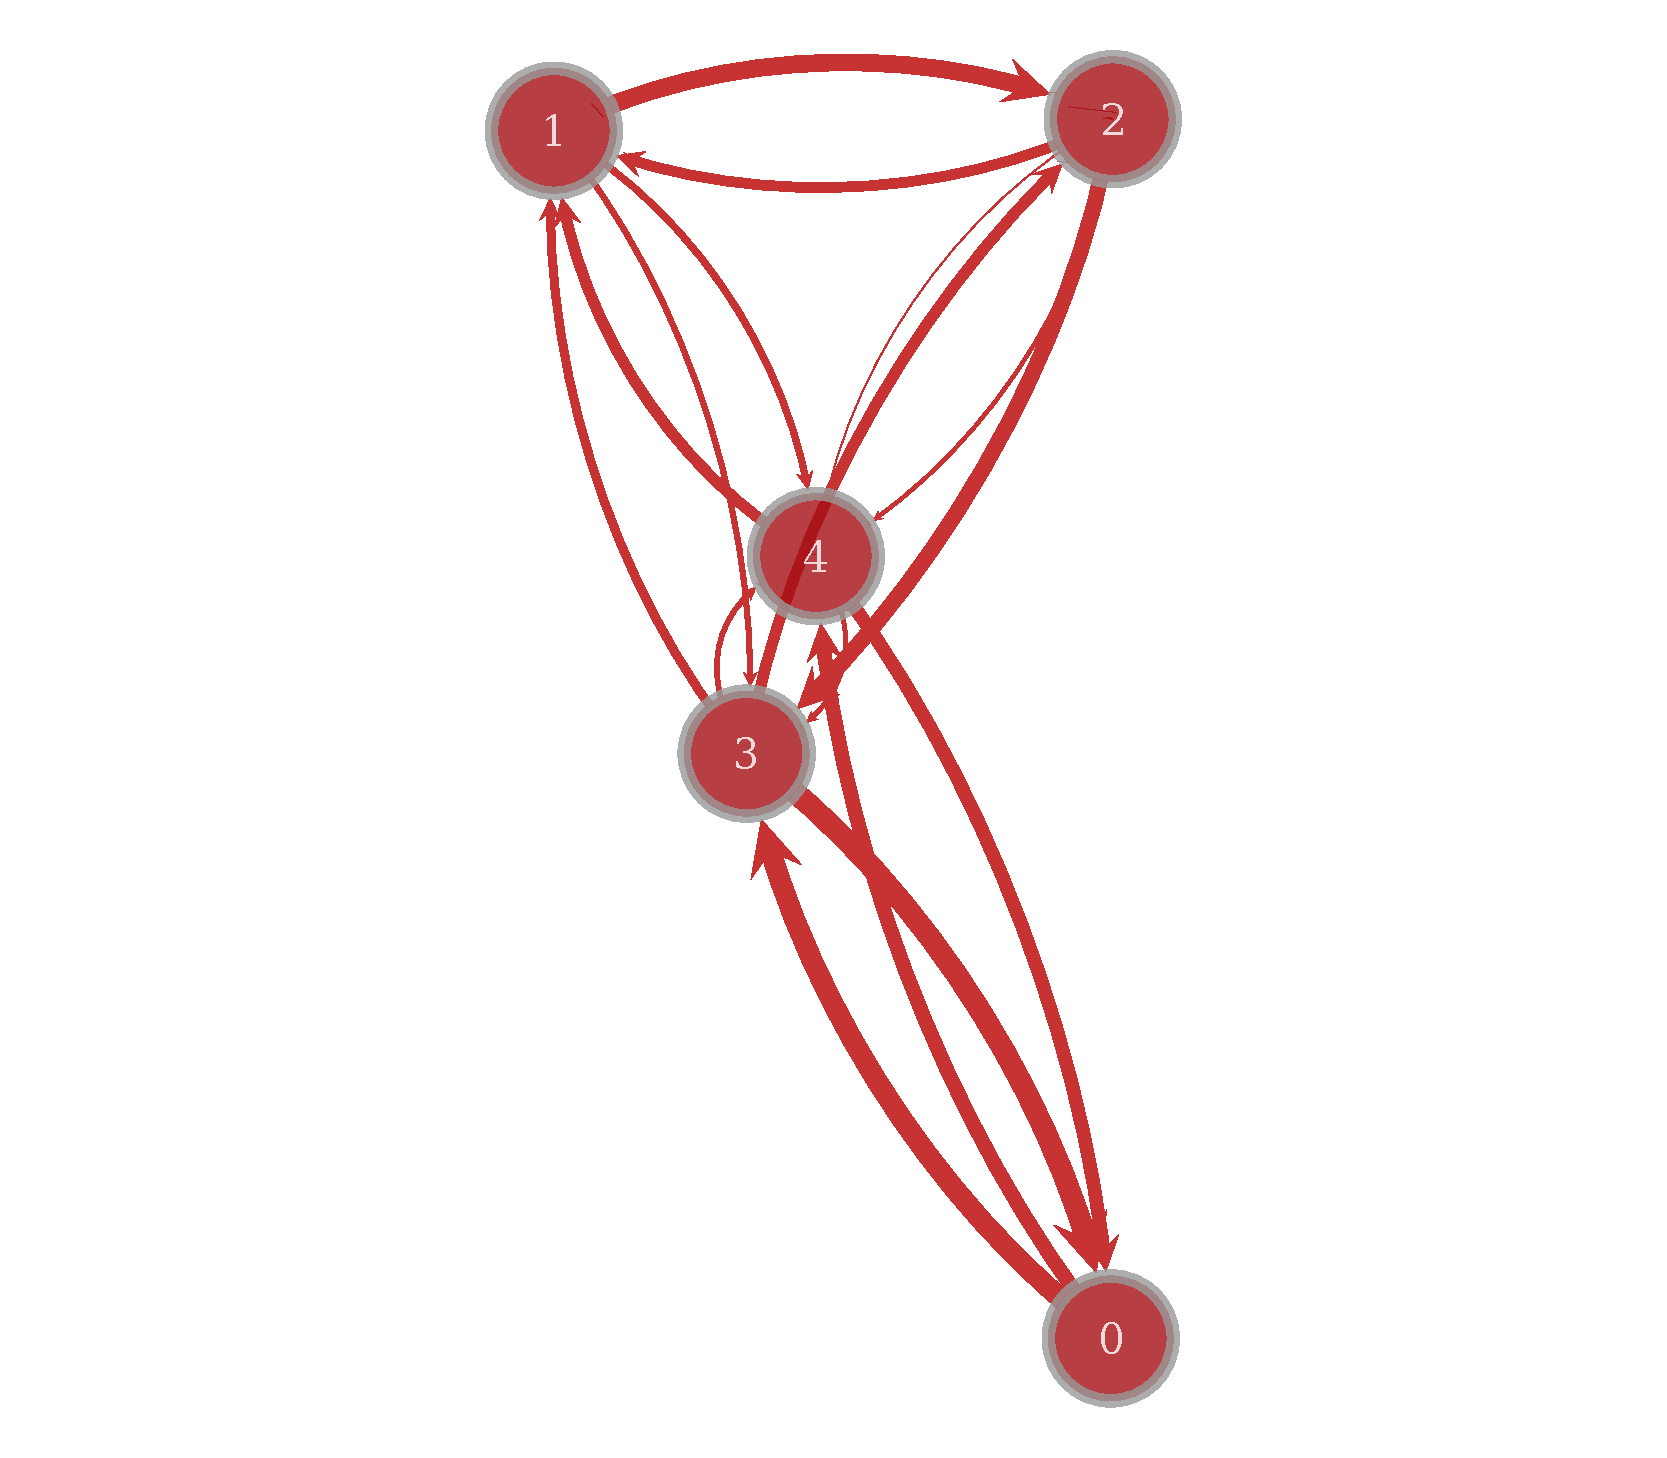
\includegraphics[width=\textwidth]{optimized_mu}
        \caption{Сетевой трафик}
        \label{fig:optimized_mu}
    \end{subfigure}
    \begin{subfigure}{0.49\textwidth}
        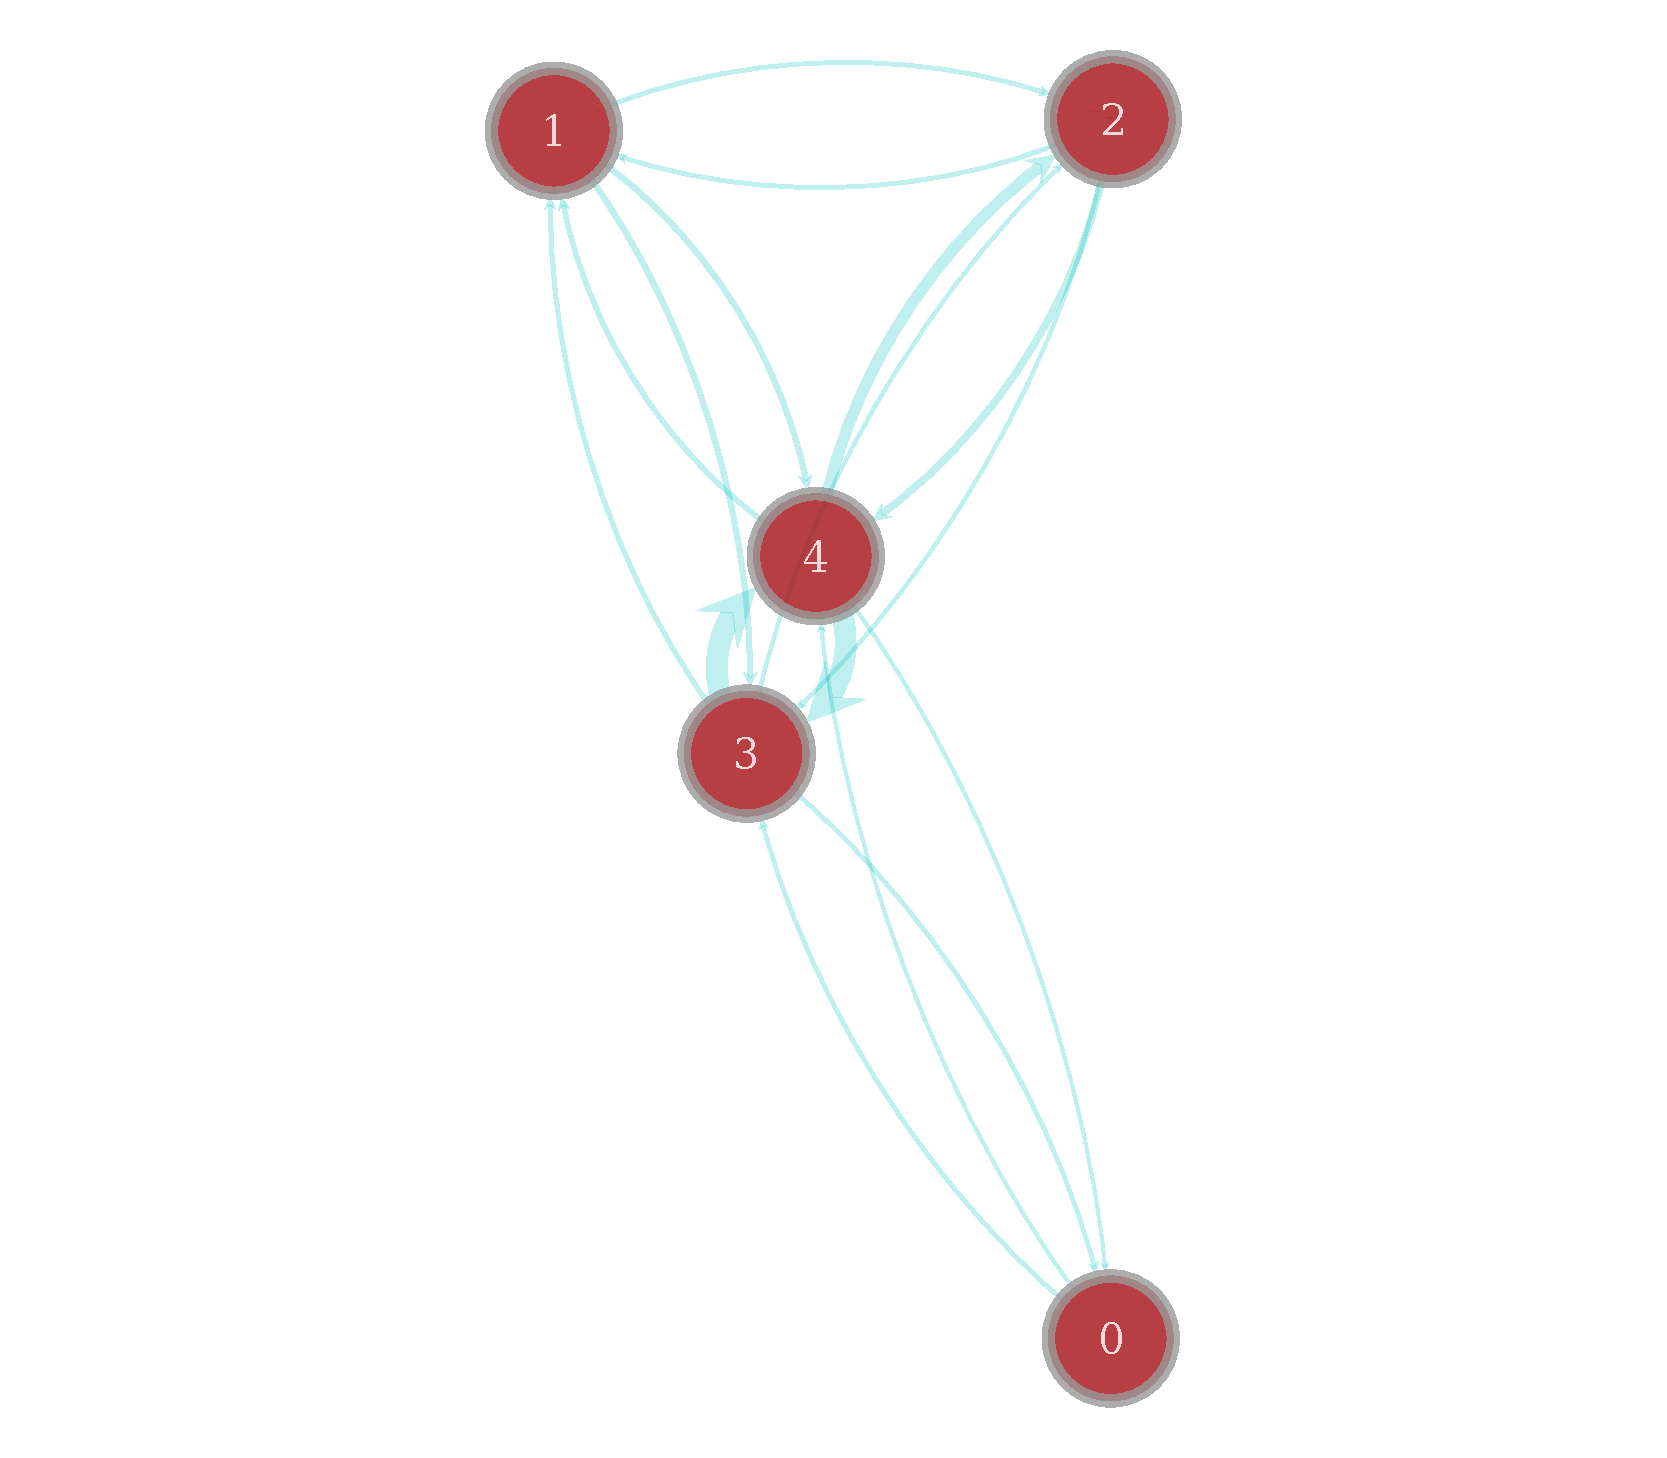
\includegraphics[width=\textwidth]{optimized_lambda}
        \caption{Емкость каналов связи}
        \label{fig:optimized_lambda}
    \end{subfigure}
    \caption{Визуализация оптимального решения}\label{fig:optimized_solution}
\end{figure}

Таким образом, получено оптимальное решение одновременно задачи маршрутизации и территориально-частотного планирования. Последовательно было найдено опорное решение, после чего информационные потоки и частотные каналы были перераспределены по критерию минимальности суммарных задержек, возникающих в сети.
\nnumsection{ЗАКЛЮЧЕНИЕ}
В результате неоднократного повторения алгоритма оптимизации для различного числа узлов и топологий было выяснено, что для достижения оптимального решения можно ограничиться небольшим количеством наиболее выгодных маршрутов, поскольку значительная часть потока данных идет через считанное число путей: на долю 1--2 маршрутов приходится около 90 \% трафика или более. Но при этом к вопросу выбора метрики следует отнестись максимально внимательно~-- не обязательно маршрут с наименьшим числом промежуточных узлов будет в итоге являться самым выгодным.

Полученное одновременное решение задачи частотного планирования и распределения трафика возвращает к дискуссии о правомерности и востребованности межуровневого подхода при построении стека протоколов связи~-- подробная информация об информационных потоках для более низких уровней может оказать значительное влияние на итоговую производительность сети. 

Управление шириной полосы частот, используемой для передачи данных, можно реализовать различными способами: например, с помощью варьирования бодовой скорости передачи данных, при использовании методов расширения спектра; в случае работы с OFDM ширина частотной полосы может регулироваться изменением количества поднесущих. В целом же проблемой адаптивности радиоканала занимается отрасль программно-определяемого и когнитивного радио.

Возможно оценить сложность задачи -- для построения опорного решения неполносвязной сети из пяти узлов необходимо получить решение для 33 линейных уравнений c 162 неизвестными, что в реальности представляется не всегда возможным за сжатый срок по причине ограниченной производительности вычислительных устройств. Поэтому при критической важности скорости получения решения и ограниченных вычислительных ресурсах следует использовать квазиоптимальные алгоритмы и эвристические методы работы с маршрутами. Но, как было отмечено выше, стремительное развитие микроэлектронной базы дает возможность для реализации в скором будущем предложенной схемы с характеристиками, соответствующими рыночным ожиданиям.

\nnumsection{ЛИТЕРАТУРА}
\begin{enumerate}
\item Akyildiz I. F., Wang X. A Survey on Wireless Mesh Networks // IEEE Radio Communications. 2005. Vol. 43. Is. 9. P. S23--S30.
\item Ramanathan R., Radi J. A brief overview of Ad Hoc Networks: challenges anddirections // IEEE Communications Magazine. 2002. Vol. 40. Is. 5. P. 20--22.
\item Cisco Meraki | Mesh routing [Электронный ресурс]. -- Режим доступа: https://meraki.cisco.com/technologies/mesh-routing (дата обращения: 01.06.16).
\item Wireless WDS Mesh -- MikroTik Wiki [Электронный ресурс]. -- Режим доступа: http://wiki.mikrotik.com/wiki/Wireless\_WDS\_Mesh (дата обращения: 01.06.16).
\item OLSR Mesh [OpenWrt Wiki] [Электронный ресурс]. -- Режим доступа: http://wiki.openwrt.org/ru/inbox/mesh.olsr (дата обращения: 01.06.16).
\item Клейнрок, Л. Вычислительные сети с очередями. Пер с англ. -- М.: Мир. 1979.
\item SciPy.org -- SciPy.org [Электронный ресурс]. -- Режим доступа: https://www.scipy.org/ (дата обращения: 01.06.16).
\item RFC 3561. Ad hoc On-Demand Distance Vector (AODV) Routing. -- введ. 07.2003. -- The Internet Engineering Task Force -- 37 с.
\item RFC 4728. The Dynamic Source Routing Protocol (DSR) for Mobile Ad Hoc Networks for IPv4. -- введ. 02.2007. -- The Internet Engineering Task Force -- 102 с.
\item RFC 3626. Optimized Link State Routing Protocol (OLSR). -- введ. 10.2003. -- The Internet Engineering Task Force -- 75 с.
\item Hoebeke J., Moerman I., Dhoedt B., Demeester P. An overview of mobile ad hoc networks: applications and challenges // 43rd European Telecommunications Congress: Proceedings Paper; 09.08.2004 / Journal of the communications network 3(3) 2004, с.60-66.
\item Dr. Pradip Ghorpade, Pravin Ghosekar, Girish Katkar. Mobile Ad Hoc Networking: Imperatives and Challenges // IJCA Special Issue on MANETs -- 2010 -- №3 -- p. 153--158, 2010. Published by Foundation of Computer Science.
\item А.П. Метелёв, А.В. Чистяков, А.Н. Жолобов. Протоколы маршрутизации в беспроводных самоорганизующихся сетях // Вестник Нижегородского университета им. Н. И. Лобачевского -- 2013 -- № 3 (1) -- С. 75-78.
\item В.М. Винокуров, А.В. Пуговкин, А.А. Пшенников, Д.Н. Ушарова, А.С. Филатов. Маршрутизация в беспроводных мобильных Ad hoc-сетях // Доклады ТУСУРа -- 2010  --  №2 (22)  --  ч.1  -- С. 288-292.
\item Аоки М. Введение в методы оптимизации. - М.: Наука, 1977. -- 334~с.
\item Сеа Ж. Оптимизация. Теория и алгоритмы. - М.: Мир, 1973.
\item Шевелев Ю. П. Дискретная математика. Ч. 2: Теория конечных автоматов. Комбинаторика. Теория графов (для автоматизированной технологии обучения «Символ»): Учебное пособие. -- Томск: Том. гос. ун-т систем упр. и радиоэлектроники, 2003. -- 130 с.
\end{enumerate}

\clearpage
\begin{center}
\textbf{ПРИЛОЖЕНИЕ А} \\
(справочное)
\end{center}
\par \addvspace{0.5\baselineskip}
\begin{minipage}{\textwidth-\parindent}
\textbf{Листинг А.1 -- Расчет оптимизационной задачи на языке программирования Python}%
\end{minipage}
\inputminted[breaklines,linenos,fontsize=\small]{python}{single_solution.py}
\end{document}